\documentclass[screen,acmsmall]{acmart}%\settopmatter{printfolios=false,printccs=false,printacmref=false}
\setcopyright{none}
\renewcommand\footnotetextcopyrightpermission[1]{}
\pagestyle{plain}

\bibliographystyle{ACM-Reference-Format}
\citestyle{acmauthoryear}   %% For author/year citations
\usepackage{listings,hyperref,multirow,paralist,xspace,url,wrapfig,tikz}
\usetikzlibrary{positioning,automata,fit,shapes.geometric,backgrounds,calc}
\usepackage{tabularx}
\newcommand{\missingTag}[1]{\textcolor{red}{#1}\xspace}
\newcommand{\missingNumber}{\textcolor{red}{XX}\xspace}
\newcommand{\missingPercentage}{\textcolor{red}{XX\%}\xspace}
\newcommand{\missingTable}[1][XX]{\textcolor{red}{Table #1}\xspace}
\newcommand{\missingGraph}{\textcolor{red}{XXGraph}\xspace}

\input{tag/corpus.tex}
\input{tag/side-effects.tex}
\input{tag/package_usage_metrics.tex}
\input{tag/kaggle_usage_metrics.tex}
\input{tag/base_usage_metrics.tex}
\newcommand{\packageNbCallSitesRnd}{17.5K\xspace}
\newcommand{\packageNbCallSites}{17,483\xspace}
\newcommand{\packageMinimizedcallsitesaRnd}{4.7K\xspace}
\newcommand{\packageMinimizedcallsitesa}{4,701\xspace}
\newcommand{\packageMinimizedcallsitesbRnd}{3.6K\xspace}
\newcommand{\packageMinimizedcallsitesb}{3,627\xspace}
\newcommand{\packageMinimizedcallsitescRnd}{2.8K\xspace}
\newcommand{\packageMinimizedcallsitesc}{2,791\xspace}
\newcommand{\packageMinimizedcallsitesdRnd}{2.2K\xspace}
\newcommand{\packageMinimizedcallsitesd}{2,181\xspace}
\newcommand{\packageMinimizedcallsiteseRnd}{1.7K\xspace}
\newcommand{\packageMinimizedcallsitese}{1,708\xspace}
\newcommand{\packageMinimizedcallsitesfRnd}{1.3K\xspace}
\newcommand{\packageMinimizedcallsitesf}{1,261\xspace}
\newcommand{\packageMinimizedcallsitesgRnd}{1.2K\xspace}
\newcommand{\packageMinimizedcallsitesg}{1,184\xspace}
\newcommand{\packageMinimizedcallsiteshRnd}{1.1K\xspace}
\newcommand{\packageMinimizedcallsitesh}{1,126\xspace}
\newcommand{\packageMinimizedcallsitesiRnd}{858\xspace}
\newcommand{\packageMinimizedcallsitesi}{858\xspace}
\newcommand{\packageMinimizedcallsitesjRnd}{731\xspace}
\newcommand{\packageMinimizedcallsitesj}{731\xspace}
\newcommand{\packageMinimizedcallsiteskRnd}{437\xspace}
\newcommand{\packageMinimizedcallsitesk}{437\xspace}
\newcommand{\packageMinimizedcallsiteslRnd}{113\xspace}
\newcommand{\packageMinimizedcallsitesl}{113\xspace}
\newcommand{\packageMinimizedpropsitesa}{27\%\xspace}
\newcommand{\packageMinimizedpropsitesb}{21\%\xspace}
\newcommand{\packageMinimizedpropsitesc}{16\%\xspace}
\newcommand{\packageMinimizedpropsitesd}{12\%\xspace}
\newcommand{\packageMinimizedpropsitese}{10\%\xspace}
\newcommand{\packageMinimizedpropsitesf}{7\%\xspace}
\newcommand{\packageMinimizedpropsitesg}{7\%\xspace}
\newcommand{\packageMinimizedpropsitesh}{6\%\xspace}
\newcommand{\packageMinimizedpropsitesi}{5\%\xspace}
\newcommand{\packageMinimizedpropsitesj}{4\%\xspace}
\newcommand{\packageMinimizedpropsitesk}{2\%\xspace}
\newcommand{\packageMinimizedpropsitesl}{0.6\%\xspace}
\newcommand{\packageMinimizedpackageaRnd}{1K\xspace}
\newcommand{\packageMinimizedpackagea}{1,012\xspace}
\newcommand{\packageMinimizedpackagebRnd}{831\xspace}
\newcommand{\packageMinimizedpackageb}{831\xspace}
\newcommand{\packageMinimizedpackagecRnd}{786\xspace}
\newcommand{\packageMinimizedpackagec}{786\xspace}
\newcommand{\packageMinimizedpackagedRnd}{768\xspace}
\newcommand{\packageMinimizedpackaged}{768\xspace}
\newcommand{\packageMinimizedpackageeRnd}{514\xspace}
\newcommand{\packageMinimizedpackagee}{514\xspace}
\newcommand{\packageMinimizedpackagefRnd}{508\xspace}
\newcommand{\packageMinimizedpackagef}{508\xspace}
\newcommand{\packageMinimizedpackagegRnd}{486\xspace}
\newcommand{\packageMinimizedpackageg}{486\xspace}
\newcommand{\packageMinimizedpackagehRnd}{129\xspace}
\newcommand{\packageMinimizedpackageh}{129\xspace}
\newcommand{\packageMinimizedpackageiRnd}{274\xspace}
\newcommand{\packageMinimizedpackagei}{274\xspace}
\newcommand{\packageMinimizedpackagejRnd}{150\xspace}
\newcommand{\packageMinimizedpackagej}{150\xspace}
\newcommand{\packageMinimizedpackagekRnd}{145\xspace}
\newcommand{\packageMinimizedpackagek}{145\xspace}
\newcommand{\packageMinimizedpackagelRnd}{67\xspace}
\newcommand{\packageMinimizedpackagel}{67\xspace}
\newcommand{\packageMinimizedoperationsaRnd}{1.2K\xspace}
\newcommand{\packageMinimizedoperationsa}{1,193\xspace}
\newcommand{\packageMinimizedoperationsbRnd}{28.3K\xspace}
\newcommand{\packageMinimizedoperationsb}{28,347\xspace}
\newcommand{\packageMinimizedoperationscRnd}{927\xspace}
\newcommand{\packageMinimizedoperationsc}{927\xspace}
\newcommand{\packageMinimizedoperationsdRnd}{5.4K\xspace}
\newcommand{\packageMinimizedoperationsd}{5,355\xspace}
\newcommand{\packageMinimizedoperationseRnd}{654\xspace}
\newcommand{\packageMinimizedoperationse}{654\xspace}
\newcommand{\packageMinimizedoperationsfRnd}{3.2K\xspace}
\newcommand{\packageMinimizedoperationsf}{3,239\xspace}
\newcommand{\packageMinimizedoperationsgRnd}{1.7K\xspace}
\newcommand{\packageMinimizedoperationsg}{1,674\xspace}
\newcommand{\packageMinimizedoperationshRnd}{56\xspace}
\newcommand{\packageMinimizedoperationsh}{56\xspace}
\newcommand{\packageMinimizedoperationsiRnd}{6.8K\xspace}
\newcommand{\packageMinimizedoperationsi}{6,830\xspace}
\newcommand{\packageMinimizedoperationsjRnd}{248.2K\xspace}
\newcommand{\packageMinimizedoperationsj}{248,166\xspace}
\newcommand{\packageMinimizedoperationskRnd}{15.2K\xspace}
\newcommand{\packageMinimizedoperationsk}{15,230\xspace}
\newcommand{\packageMinimizedoperationslRnd}{96.9K\xspace}
\newcommand{\packageMinimizedoperationsl}{96,867\xspace}
\newcommand{\packageMinimizedmedianoperationsaRnd}{5\xspace}
\newcommand{\packageMinimizedmedianoperationsa}{5\xspace}
\newcommand{\packageMinimizedmedianoperationsbRnd}{81\xspace}
\newcommand{\packageMinimizedmedianoperationsb}{81\xspace}
\newcommand{\packageMinimizedmedianoperationscRnd}{2\xspace}
\newcommand{\packageMinimizedmedianoperationsc}{2\xspace}
\newcommand{\packageMinimizedmedianoperationsdRnd}{16\xspace}
\newcommand{\packageMinimizedmedianoperationsd}{16\xspace}
\newcommand{\packageMinimizedmedianoperationseRnd}{8\xspace}
\newcommand{\packageMinimizedmedianoperationse}{8\xspace}
\newcommand{\packageMinimizedmedianoperationsfRnd}{1.9K\xspace}
\newcommand{\packageMinimizedmedianoperationsf}{1,929\xspace}
\newcommand{\packageMinimizedmedianoperationsgRnd}{95\xspace}
\newcommand{\packageMinimizedmedianoperationsg}{95\xspace}
\newcommand{\packageMinimizedmedianoperationshRnd}{10\xspace}
\newcommand{\packageMinimizedmedianoperationsh}{10\xspace}
\newcommand{\packageMinimizedmedianoperationsiRnd}{60\xspace}
\newcommand{\packageMinimizedmedianoperationsi}{60\xspace}
\newcommand{\packageMinimizedmedianoperationsjRnd}{5K\xspace}
\newcommand{\packageMinimizedmedianoperationsj}{4,967.5\xspace}
\newcommand{\packageMinimizedmedianoperationskRnd}{70\xspace}
\newcommand{\packageMinimizedmedianoperationsk}{70\xspace}
\newcommand{\packageMinimizedmedianoperationslRnd}{11.6K\xspace}
\newcommand{\packageMinimizedmedianoperationsl}{11,642\xspace}
\newcommand{\packageMinimizedpercentenvira}{73\%\xspace}
\newcommand{\packageMinimizedpercentenvirb}{61\%\xspace}
\newcommand{\packageMinimizedpercentenvirc}{62\%\xspace}
\newcommand{\packageMinimizedpercentenvird}{56\%\xspace}
\newcommand{\packageMinimizedpercentenvire}{47\%\xspace}
\newcommand{\packageMinimizedpercentenvirf}{80\%\xspace}
\newcommand{\packageMinimizedpercentenvirg}{45\%\xspace}
\newcommand{\packageMinimizedpercentenvirh}{82\%\xspace}
\newcommand{\packageMinimizedpercentenviri}{24\%\xspace}
\newcommand{\packageMinimizedpercentenvirj}{44\%\xspace}
\newcommand{\packageMinimizedpercentenvirk}{35\%\xspace}
\newcommand{\packageMinimizedpercentenvirl}{47\%\xspace}
\newcommand{\packageMinimizedpercentcallsenvira}{81\%\xspace}
\newcommand{\packageMinimizedpercentcallsenvirb}{47\%\xspace}
\newcommand{\packageMinimizedpercentcallsenvirc}{59\%\xspace}
\newcommand{\packageMinimizedpercentcallsenvird}{68\%\xspace}
\newcommand{\packageMinimizedpercentcallsenvire}{60\%\xspace}
\newcommand{\packageMinimizedpercentcallsenvirf}{72\%\xspace}
\newcommand{\packageMinimizedpercentcallsenvirg}{19\%\xspace}
\newcommand{\packageMinimizedpercentcallsenvirh}{18\%\xspace}
\newcommand{\packageMinimizedpercentcallsenviri}{8\%\xspace}
\newcommand{\packageMinimizedpercentcallsenvirj}{74\%\xspace}
\newcommand{\packageMinimizedpercentcallsenvirk}{10\%\xspace}
\newcommand{\packageMinimizedpercentcallsenvirl}{21\%\xspace}
\newcommand{\packageMinimizedpercentenvirnonparenta}{55\%\xspace}
\newcommand{\packageMinimizedpercentenvirnonparentb}{21\%\xspace}
\newcommand{\packageMinimizedpercentenvirnonparentc}{37\%\xspace}
\newcommand{\packageMinimizedpercentenvirnonparentd}{37\%\xspace}
\newcommand{\packageMinimizedpercentenvirnonparente}{28\%\xspace}
\newcommand{\packageMinimizedpercentenvirnonparentf}{14\%\xspace}
\newcommand{\packageMinimizedpercentenvirnonparentg}{28\%\xspace}
\newcommand{\packageMinimizedpercentenvirnonparenth}{6\%\xspace}
\newcommand{\packageMinimizedpercentenvirnonparenti}{21\%\xspace}
\newcommand{\packageMinimizedpercentenvirnonparentj}{19\%\xspace}
\newcommand{\packageMinimizedpercentenvirnonparentk}{13\%\xspace}
\newcommand{\packageMinimizedpercentenvirnonparentl}{38\%\xspace}
\newcommand{\packageMinimizedpercentparentframesa}{48\%\xspace}
\newcommand{\packageMinimizedpercentparentframesb}{79\%\xspace}
\newcommand{\packageMinimizedpercentparentframesc}{71\%\xspace}
\newcommand{\packageMinimizedpercentparentframesd}{68\%\xspace}
\newcommand{\packageMinimizedpercentparentframese}{79\%\xspace}
\newcommand{\packageMinimizedpercentparentframesf}{46\%\xspace}
\newcommand{\packageMinimizedpercentparentframesg}{77\%\xspace}
\newcommand{\packageMinimizedpercentparentframesh}{96\%\xspace}
\newcommand{\packageMinimizedpercentparentframesi}{78\%\xspace}
\newcommand{\packageMinimizedpercentparentframesj}{84\%\xspace}
\newcommand{\packageMinimizedpercentparentframesk}{87\%\xspace}
\newcommand{\packageMinimizedpercentparentframesl}{79\%\xspace}
\newcommand{\packageNbSimpleMinimizedOneRnd}{7.2K\xspace}
\newcommand{\packageNbSimpleMinimizedOne}{7,217\xspace}
\newcommand{\packageNbSimpleMinimizedMoreRnd}{601\xspace}
\newcommand{\packageNbSimpleMinimizedMore}{601\xspace}
\newcommand{\packageNbSymbolVarSitesRnd}{2.3K\xspace}
\newcommand{\packageNbSymbolVarSites}{2,349\xspace}
\newcommand{\packageNbSymbolVarSitePercent}{50\%\xspace}
\newcommand{\packageNbNonDefaultEnvirVariablesPercent}{82.5\%\xspace}
\newcommand{\packageFunctionDefinitionSitesRnd}{1.1K\xspace}
\newcommand{\packageFunctionDefinitionSites}{1,126\xspace}
\newcommand{\packageFunctionDefinitionSitesPercent}{6.4\%\xspace}
\newcommand{\packageFundefNonDefaultEnvirSitesPercent}{82.4\%\xspace}
\newcommand{\packageGeneralizedFunctionDefinitionSitesRnd}{1.8K\xspace}
\newcommand{\packageGeneralizedFunctionDefinitionSites}{1,753\xspace}
\newcommand{\packageGeneralizedFunctionDefinitionSitesPercent}{10\%\xspace}
\newcommand{\packageGeneralizedFundedNonDefaultEnvirSitesPercent}{52.9\%\xspace}
\newcommand{\packageNbAssignSitesRnd}{1.2K\xspace}
\newcommand{\packageNbAssignSites}{1,245\xspace}
\newcommand{\packageAssignSitesPercent}{7.1\%\xspace}
\newcommand{\packageNonDefaultEnvirAssignSitesRnd}{339\xspace}
\newcommand{\packageNonDefaultEnvirAssignSites}{339\xspace}
\newcommand{\packageNonDefaultEnvirAssignSitesPercent}{27.2\%\xspace}
\newcommand{\packageNbOneMinimizedRnd}{15.3K\xspace}
\newcommand{\packageNbOneMinimized}{15,307\xspace}
\newcommand{\packageNbOneMinimizedPercent}{87.6\%\xspace}
\newcommand{\packageNbCallSitesUniqueActualValueRnd}{1.4K\xspace}
\newcommand{\packageNbCallSitesUniqueActualValue}{1,436\xspace}
\newcommand{\packageCallSitesUniqueActualValuePercent}{51.5\%\xspace}
\newcommand{\packageMedianRunSitesUniqueActualValueRnd}{2\xspace}
\newcommand{\packageMedianRunSitesUniqueActualValue}{2\xspace}
\newcommand{\packageAverageRunSitesUniqueActualValueRnd}{14\xspace}
\newcommand{\packageAverageRunSitesUniqueActualValue}{14\xspace}
\newcommand{\packageSdRunSitesUniqueActualValueRnd}{57.9\xspace}
\newcommand{\packageSdRunSitesUniqueActualValue}{57.9\xspace}
\newcommand{\packageValOneNodeRnd}{2.2K\xspace}
\newcommand{\packageValOneNode}{2,228\xspace}
\newcommand{\packageValOneNodePercent}{74.6\%\xspace}
\newcommand{\packageOneValMedianRunsRnd}{2\xspace}
\newcommand{\packageOneValMedianRuns}{2\xspace}
\newcommand{\packageOneValAverageRunsRnd}{32.7\xspace}
\newcommand{\packageOneValAverageRuns}{32.7\xspace}
\newcommand{\packageOneValSdRunsRnd}{695\xspace}
\newcommand{\packageOneValSdRuns}{695\xspace}
\newcommand{\packageNonDefaultEnvirValuePercent}{64.1\%\xspace}
\newcommand{\packageNonDefaultEnvirWithVarPercent}{34.7\%\xspace}
\newcommand{\packageNbSlotAccessRnd}{1.7K\xspace}
\newcommand{\packageNbSlotAccess}{1,708\xspace}
\newcommand{\packageSlotAccessPercent}{9.8\%\xspace}
\newcommand{\packageGeneralizedSlotAccessRnd}{3K\xspace}
\newcommand{\packageGeneralizedSlotAccess}{3,019\xspace}
\newcommand{\packageGeneralizedSlotAccessPercent}{17.3\%\xspace}
\newcommand{\packageNdefaultEnvirSlotSiteRnd}{1.3K\xspace}
\newcommand{\packageNdefaultEnvirSlotSite}{1,306\xspace}
\newcommand{\packageNdefaultEnvirSlotSitePercent}{43.3\%\xspace}
\newcommand{\packageGeneralizedVarAccessSitesRnd}{7.6K\xspace}
\newcommand{\packageGeneralizedVarAccessSites}{7,635\xspace}
\newcommand{\packageGeneralizedVarAccessSitePercent}{43.7\%\xspace}

\input{tag/kaggle_normalized_expr.tex}
\input{tag/base_normalized_expr.tex}
\input{tag/package_environments.tex}
%\input{tag/package_provenance.tex}
\newcommand{\packageNbProvenanceCallsaRnd}{23.5M\xspace}
\newcommand{\packageNbProvenanceCallsa}{23,478,269\xspace}
\newcommand{\packageNbProvenanceCallsbRnd}{8.5M\xspace}
\newcommand{\packageNbProvenanceCallsb}{8,458,959\xspace}
\newcommand{\packageNbProvenanceCallscRnd}{3M\xspace}
\newcommand{\packageNbProvenanceCallsc}{3,042,180\xspace}
\newcommand{\packageNbProvenanceCallsdRnd}{2.3M\xspace}
\newcommand{\packageNbProvenanceCallsd}{2,318,201\xspace}
\newcommand{\packageNbProvenanceCallseRnd}{1.4M\xspace}
\newcommand{\packageNbProvenanceCallse}{1,359,948\xspace}
\newcommand{\packageNbProvenanceCallsfRnd}{1.1M\xspace}
\newcommand{\packageNbProvenanceCallsf}{1,141,083\xspace}
\newcommand{\packageNbProvenanceCallsgRnd}{704.9K\xspace}
\newcommand{\packageNbProvenanceCallsg}{704,853\xspace}
\newcommand{\packageNbProvenanceCallshRnd}{647.3K\xspace}
\newcommand{\packageNbProvenanceCallsh}{647,295\xspace}
\newcommand{\packageNbProvenanceCallsiRnd}{543.8K\xspace}
\newcommand{\packageNbProvenanceCallsi}{543,759\xspace}
\newcommand{\packageNbProvenanceCallsjRnd}{542.6K\xspace}
\newcommand{\packageNbProvenanceCallsj}{542,581\xspace}
\newcommand{\packagePercentProvenanceCallsaRnd}{53.9\xspace}
\newcommand{\packagePercentProvenanceCallsa}{53.9\xspace}
\newcommand{\packagePercentProvenanceCallsbRnd}{19.4\xspace}
\newcommand{\packagePercentProvenanceCallsb}{19.4\xspace}
\newcommand{\packagePercentProvenanceCallscRnd}{7\xspace}
\newcommand{\packagePercentProvenanceCallsc}{7\xspace}
\newcommand{\packagePercentProvenanceCallsdRnd}{5.3\xspace}
\newcommand{\packagePercentProvenanceCallsd}{5.3\xspace}
\newcommand{\packagePercentProvenanceCallseRnd}{3.1\xspace}
\newcommand{\packagePercentProvenanceCallse}{3.1\xspace}
\newcommand{\packagePercentProvenanceCallsfRnd}{2.6\xspace}
\newcommand{\packagePercentProvenanceCallsf}{2.6\xspace}
\newcommand{\packagePercentProvenanceCallsgRnd}{1.6\xspace}
\newcommand{\packagePercentProvenanceCallsg}{1.6\xspace}
\newcommand{\packagePercentProvenanceCallshRnd}{1.5\xspace}
\newcommand{\packagePercentProvenanceCallsh}{1.5\xspace}
\newcommand{\packagePercentProvenanceCallsiRnd}{1.2\xspace}
\newcommand{\packagePercentProvenanceCallsi}{1.2\xspace}
\newcommand{\packagePercentProvenanceCallsjRnd}{1.2\xspace}
\newcommand{\packagePercentProvenanceCallsj}{1.2\xspace}
\newcommand{\packageCumpercentProvenanceCallsaRnd}{53.9\xspace}
\newcommand{\packageCumpercentProvenanceCallsa}{53.9\xspace}
\newcommand{\packageCumpercentProvenanceCallsbRnd}{73.4\xspace}
\newcommand{\packageCumpercentProvenanceCallsb}{73.4\xspace}
\newcommand{\packageCumpercentProvenanceCallscRnd}{80.4\xspace}
\newcommand{\packageCumpercentProvenanceCallsc}{80.4\xspace}
\newcommand{\packageCumpercentProvenanceCallsdRnd}{85.7\xspace}
\newcommand{\packageCumpercentProvenanceCallsd}{85.7\xspace}
\newcommand{\packageCumpercentProvenanceCallseRnd}{88.8\xspace}
\newcommand{\packageCumpercentProvenanceCallse}{88.8\xspace}
\newcommand{\packageCumpercentProvenanceCallsfRnd}{91.4\xspace}
\newcommand{\packageCumpercentProvenanceCallsf}{91.4\xspace}
\newcommand{\packageCumpercentProvenanceCallsgRnd}{93.1\xspace}
\newcommand{\packageCumpercentProvenanceCallsg}{93.1\xspace}
\newcommand{\packageCumpercentProvenanceCallshRnd}{94.5\xspace}
\newcommand{\packageCumpercentProvenanceCallsh}{94.5\xspace}
\newcommand{\packageCumpercentProvenanceCallsiRnd}{95.8\xspace}
\newcommand{\packageCumpercentProvenanceCallsi}{95.8\xspace}
\newcommand{\packageCumpercentProvenanceCallsjRnd}{97\xspace}
\newcommand{\packageCumpercentProvenanceCallsj}{97\xspace}
\newcommand{\packageProvenanceNamea}{parse\xspace}
\newcommand{\packageProvenanceNameb}{substitute\xspace}
\newcommand{\packageProvenanceNamec}{match.call\xspace}
\newcommand{\packageProvenanceNamed}{NA\xspace}
\newcommand{\packageProvenanceNamee}{expression\xspace}
\newcommand{\packageProvenanceNamef}{quote\xspace}
\newcommand{\packageProvenanceNameg}{as.name\xspace}
\newcommand{\packageProvenanceNameh}{call\xspace}
\newcommand{\packageProvenanceNamei}{as.call\xspace}
\newcommand{\packageProvenanceNamej}{[[\xspace}
\newcommand{\packageProvenanceNamek}{\$\xspace}
\newcommand{\packageProvenanceNamel}{.External\xspace}
\newcommand{\packageProvenanceNamem}{as.vector\xspace}
\newcommand{\packageProvenanceNamen}{formals\xspace}
\newcommand{\packageNbProvenanceSitesaRnd}{4K\xspace}
\newcommand{\packageNbProvenanceSitesa}{4,006\xspace}
\newcommand{\packageNbProvenanceSitesbRnd}{3.9K\xspace}
\newcommand{\packageNbProvenanceSitesb}{3,916\xspace}
\newcommand{\packageNbProvenanceSitescRnd}{2.1K\xspace}
\newcommand{\packageNbProvenanceSitesc}{2,058\xspace}
\newcommand{\packageNbProvenanceSitesdRnd}{1.1K\xspace}
\newcommand{\packageNbProvenanceSitesd}{1,116\xspace}
\newcommand{\packageNbProvenanceSiteseRnd}{597\xspace}
\newcommand{\packageNbProvenanceSitese}{597\xspace}
\newcommand{\packageNbProvenanceSitesfRnd}{557\xspace}
\newcommand{\packageNbProvenanceSitesf}{557\xspace}
\newcommand{\packageNbProvenanceSitesgRnd}{482\xspace}
\newcommand{\packageNbProvenanceSitesg}{482\xspace}
\newcommand{\packageNbProvenanceSiteshRnd}{475\xspace}
\newcommand{\packageNbProvenanceSitesh}{475\xspace}
\newcommand{\packageNbProvenanceSitesiRnd}{450\xspace}
\newcommand{\packageNbProvenanceSitesi}{450\xspace}
\newcommand{\packageNbProvenanceSitesjRnd}{364\xspace}
\newcommand{\packageNbProvenanceSitesj}{364\xspace}
\newcommand{\packageNbProvenanceSiteskRnd}{271\xspace}
\newcommand{\packageNbProvenanceSitesk}{271\xspace}
\newcommand{\packageNbProvenanceSiteslRnd}{251\xspace}
\newcommand{\packageNbProvenanceSitesl}{251\xspace}
\newcommand{\packageNbProvenanceSitesmRnd}{210\xspace}
\newcommand{\packageNbProvenanceSitesm}{210\xspace}
\newcommand{\packageNbProvenanceSitesnRnd}{112\xspace}
\newcommand{\packageNbProvenanceSitesn}{112\xspace}
\newcommand{\packagePercentProvenanceSitesaRnd}{22.9\xspace}
\newcommand{\packagePercentProvenanceSitesa}{22.9\xspace}
\newcommand{\packagePercentProvenanceSitesbRnd}{22.4\xspace}
\newcommand{\packagePercentProvenanceSitesb}{22.4\xspace}
\newcommand{\packagePercentProvenanceSitescRnd}{11.8\xspace}
\newcommand{\packagePercentProvenanceSitesc}{11.8\xspace}
\newcommand{\packagePercentProvenanceSitesdRnd}{6.4\xspace}
\newcommand{\packagePercentProvenanceSitesd}{6.4\xspace}
\newcommand{\packagePercentProvenanceSiteseRnd}{3.4\xspace}
\newcommand{\packagePercentProvenanceSitese}{3.4\xspace}
\newcommand{\packagePercentProvenanceSitesfRnd}{3.2\xspace}
\newcommand{\packagePercentProvenanceSitesf}{3.2\xspace}
\newcommand{\packagePercentProvenanceSitesgRnd}{2.8\xspace}
\newcommand{\packagePercentProvenanceSitesg}{2.8\xspace}
\newcommand{\packagePercentProvenanceSiteshRnd}{2.7\xspace}
\newcommand{\packagePercentProvenanceSitesh}{2.7\xspace}
\newcommand{\packagePercentProvenanceSitesiRnd}{2.6\xspace}
\newcommand{\packagePercentProvenanceSitesi}{2.6\xspace}
\newcommand{\packagePercentProvenanceSitesjRnd}{2.1\xspace}
\newcommand{\packagePercentProvenanceSitesj}{2.1\xspace}
\newcommand{\packagePercentProvenanceSiteskRnd}{1.6\xspace}
\newcommand{\packagePercentProvenanceSitesk}{1.6\xspace}
\newcommand{\packagePercentProvenanceSiteslRnd}{1.4\xspace}
\newcommand{\packagePercentProvenanceSitesl}{1.4\xspace}
\newcommand{\packagePercentProvenanceSitesmRnd}{1.2\xspace}
\newcommand{\packagePercentProvenanceSitesm}{1.2\xspace}
\newcommand{\packagePercentProvenanceSitesnRnd}{0.6\xspace}
\newcommand{\packagePercentProvenanceSitesn}{0.6\xspace}
\newcommand{\packageCumpercentProvenanceSitesaRnd}{22.9\xspace}
\newcommand{\packageCumpercentProvenanceSitesa}{22.9\xspace}
\newcommand{\packageCumpercentProvenanceSitesbRnd}{45.3\xspace}
\newcommand{\packageCumpercentProvenanceSitesb}{45.3\xspace}
\newcommand{\packageCumpercentProvenanceSitescRnd}{57.1\xspace}
\newcommand{\packageCumpercentProvenanceSitesc}{57.1\xspace}
\newcommand{\packageCumpercentProvenanceSitesdRnd}{63.5\xspace}
\newcommand{\packageCumpercentProvenanceSitesd}{63.5\xspace}
\newcommand{\packageCumpercentProvenanceSiteseRnd}{66.9\xspace}
\newcommand{\packageCumpercentProvenanceSitese}{66.9\xspace}
\newcommand{\packageCumpercentProvenanceSitesfRnd}{70.1\xspace}
\newcommand{\packageCumpercentProvenanceSitesf}{70.1\xspace}
\newcommand{\packageCumpercentProvenanceSitesgRnd}{72.8\xspace}
\newcommand{\packageCumpercentProvenanceSitesg}{72.8\xspace}
\newcommand{\packageCumpercentProvenanceSiteshRnd}{75.5\xspace}
\newcommand{\packageCumpercentProvenanceSitesh}{75.5\xspace}
\newcommand{\packageCumpercentProvenanceSitesiRnd}{78.1\xspace}
\newcommand{\packageCumpercentProvenanceSitesi}{78.1\xspace}
\newcommand{\packageCumpercentProvenanceSitesjRnd}{80.2\xspace}
\newcommand{\packageCumpercentProvenanceSitesj}{80.2\xspace}
\newcommand{\packageCumpercentProvenanceSiteskRnd}{81.7\xspace}
\newcommand{\packageCumpercentProvenanceSitesk}{81.7\xspace}
\newcommand{\packageCumpercentProvenanceSiteslRnd}{83.2\xspace}
\newcommand{\packageCumpercentProvenanceSitesl}{83.2\xspace}
\newcommand{\packageCumpercentProvenanceSitesmRnd}{84.4\xspace}
\newcommand{\packageCumpercentProvenanceSitesm}{84.4\xspace}
\newcommand{\packageCumpercentProvenanceSitesnRnd}{85\xspace}
\newcommand{\packageCumpercentProvenanceSitesn}{85\xspace}
\newcommand{\packageNbStringSitesRnd}{4.1K\xspace}
\newcommand{\packageNbStringSites}{4,107\xspace}
\newcommand{\packageStringSitesPercent}{23.5\%\xspace}
\newcommand{\packageNbReflectionSitesRnd}{7.9K\xspace}
\newcommand{\packageNbReflectionSites}{7,857\xspace}
\newcommand{\packageReflectionSitesPercent}{44.9\%\xspace}
\newcommand{\packageNbConstructedSitesRnd}{3.1K\xspace}
\newcommand{\packageNbConstructedSites}{3,086\xspace}
\newcommand{\packageConstructedSitesPercent}{17.7\%\xspace}
\newcommand{\packageNbSymbolSitesRnd}{1.2K\xspace}
\newcommand{\packageNbSymbolSites}{1,200\xspace}
\newcommand{\packageSymbolSitesPercent}{6.9\%\xspace}
\newcommand{\packageNbExternalSitesRnd}{278\xspace}
\newcommand{\packageNbExternalSites}{278\xspace}
\newcommand{\packageExternalSitesPercent}{1.6\%\xspace}
\newcommand{\packageNbParseFromFileSitesRnd}{11\xspace}
\newcommand{\packageNbParseFromFileSites}{11\xspace}

\input{tag/kaggle_provenance.tex}

\graphicspath{{img/}}

\lstset{language=R}

\definecolor{LightGray}{rgb}{.92,.92,.92}
\definecolor{Gray}{rgb}{.3,.3,.3}
\definecolor{DarkGray}{rgb}{.5,.5,.5}

\lstset{ %
  columns=flexible,
  captionpos=b,
  frame=single,
  framerule=0pt,
  framexleftmargin=-1mm,
  framexrightmargin=-1mm,
  tabsize=2,
  belowskip=0pt,
  basicstyle=\small\ttfamily,
  backgroundcolor=\color{LightGray},
  keywordstyle=\small\ttfamily\bfseries,
  commentstyle=\color{Gray}\em,
  stringstyle=\color{DarkGray}, %
  literate={<-}{{$\leftarrow$\,}}1{<<-}{{$\twoheadleftarrow$}}1,
  keywords={new, env, call, eval, evalq, function, local, parent, quote
            return, ifelse, for, in, frame, basenv},
}

\lstdefinestyle{R}{ language=R, breaklines=true }

\newcommand{\eg}{\emph{e.g.},\xspace\xspace}
\newcommand{\ie}{\emph{i.e.},\xspace}
\newcommand{\cf}{\emph{cf.}\xspace}
\newcommand{\summary}[1]{{\csname #1\endcsname} ({\csname #1Min\endcsname} / {\csname #1Mean\endcsname} / {\csname #1Max\endcsname})}
\newcommand{\summaryrnd}[1]{{\csname #1Rnd\endcsname} ({\csname #1MinRnd\endcsname} / {\csname #1MeanRnd\endcsname} / {\csname #1MaxRnd\endcsname})}

\newcommand{\eval}{\texttt{eval}\xspace}
\newcommand{\Eval}{\texttt{Eval}\xspace}
\newcommand{\evals}{{\sf eval}s\xspace}
\newcommand{\parse}{\c{parse}}
\newcommand{\source}{\c{source}}
\newcommand{\local}{\c{local}}
\newcommand{\unlockBinding}{\c{unlockBinding}}
\newcommand{\substitute}{\c{substitute}}
\newcommand{\datatable}{\c{data.table}}
\newcommand{\mlogit}{\c{mlogit}}
\newcommand{\mboost}{\c{mboost}}
\newcommand{\metafor}{\c{metafor}}
\newcommand{\lavaan}{\c{lavaan}}
\newcommand{\mclust}{\c{mclust}}
\newcommand{\gamlss}{\c{gamlss}}
\newcommand{\ggproto}{\c{ggproto}}
\newcommand{\ggplot}{\c{ggplot2}}
\newcommand{\base}{\c{base}}
\renewcommand{\c}[1]{{\sf #1}\xspace}
\newcommand{\miss}[1]{{\textcolor{red}{#1}}\xspace}
\newcommand{\evil}{\emph{evil}\xspace}
\newcommand{\instrumentr}{\emph{instrumentr}\xspace}
\newcommand{\rdyntrace}{\emph{R-dyntrace}\xspace}
\newcommand{\covr}{\emph{covr}\xspace}
\newcommand{\runr}{\emph{runr}\xspace}
\newcommand{\genthat}{\emph{genthat}\xspace}

\newcommand{\NOTE}[1]{{\it Note: #1}\xspace}
\newcommand{\authorcomment}[3]{\xspace\textcolor{#1}{{\bf #2} #3}\xspace}
\newcommand{\todo}[1]{\authorcomment{red}{TODO}{#1}}
\renewcommand{\k}[1]{\lstinline |#1|\xspace}
% cf. https://tex.stackexchange.com/a/144640
\makeatletter\let\expandableinput\@@input\makeatother
\lstdefinelanguage{smalleR} {
  morekeywords={
    for,
    if,
    else,
    function
  },
  sensitive=true, % keywords are not case-sensitive
  morecomment=[l]{\#}, % l is for line comment
  morestring=[b]{"} % defines that strings are enclosed in double quotes
}
\lstset{
  language={smalleR},
  columns=flexible,
  captionpos=b,
  frame=single,
  framerule=0pt,
%  framexleftmargin=1mm,
%  framexrightmargin=1mm,
  tabsize=2,
  belowskip=0pt,
  basicstyle=\small\ttfamily,
  backgroundcolor=\color{LightGray},
  emphstyle=\sffamily,
  keywordstyle=\bfseries,
  commentstyle=\color{Gray}\em,
  stringstyle=\color{Gray},
  alsoletter={., _, $},
  breaklines=true
}

\begin{document}
\title{What We Eval in the Shadows}
\subtitle{A Large-scale Study of Eval in R programs}

\author{Aviral Goel}\affiliation{\institution{Northeastern
    University}\country{USA}}
\author{Pierre Donat-Bouillud}\affiliation{\institution{Czech Technical University in Prague}\country{Czech Republic}}
\author{Filip Křikava}\affiliation{\institution{Czech Technical University in Prague}\country{Czech Republic}}
\author{Christoph Kirsch}\affiliation{\institution{Czech Technical University in Prague}\country{Czech Republic}}
\author{Jan Vitek}\affiliation{\institution{Northeastern University}\country{USA}}
\affiliation{\institution{Czech Technical University in Prague}\country{Czech Republic}}

\begin{abstract}
 Most dynamic languages allow users to turn text into code using
  various functions, often named \eval, with language-dependent semantics. The
  widespread use of these reflective functions hinders static analysis and
  prevents compilers from performing optimizations. This paper aims to provide a
  better sense of why programmers use \eval. Understanding why \eval is used in
  practice is key to finding ways to mitigate its negative impact. We have
  reasons to believe that reflective feature usage is language and application
  domain-specific; we focus on data science code written in R and compare our
  results to previous work that analyzed web programming in JavaScript. This
  paper studied \CranRunnableScripts scripts extracted from \CranPackages R
  packages, for a total of \packageAllcalls calls to \eval. We find that \eval
  is indeed in widespread use; R's \eval is more pervasive and arguably
  dangerous than what was previously reported for JavaScript.
\end{abstract}

\maketitle
\renewcommand{\shortauthors}{Goel et al.}
\renewcommand{\shorttitle}{What We Eval in the Shadows}

\section{Introduction}

Most dynamic languages provide their users with a facility to transform
unstructured text into executable code and evaluate that code. We refer to this
reflective facility as \eval bowing to its origins in LISP, all the way back in
1956. \Eval has been much maligned over the years. In computing lore, it is as
close to a boogeyman as it gets. Yet, for McCarthy, \eval was simply the way to
write down the definition of LISP; he was surprised that someone coded it up and
offered it to end users~\cite{lisp}. Since then, reflective facilities have been
used to parameterize programs over code patterns that can be provided after the
program is written. The presence of such a feature in a language is a hallmark
of dynamism; it is a form of delayed binding as the behavior of any particular
call to \eval will only be known when the program is run, and that particular
call site is evaluated.

\paragraph{Trouble in Paradise.} Reflective facilities hinder
most attempts to reason about or apply meaning-preserving transformations to the
code using them. In practice, \eval causes static analysis techniques to lose so
much precision as to become pointless. For compilers, anything but the most
trivial, local optimizations are unsound after use of \eval. Furthermore, the
addition of arbitrary code --- code that could have been obtained from a network
connection --- as a program is running is a security vulnerability waiting to
happen. To illustrate these challenges, consider the interaction of a static
analysis tool with a dynamic language. A program analyzer computes an
over-approximation of the set of possible behaviors exhibited by the program
under study, a reflective facility must be represented by all behaviors that can
be expressed in the target language. \ie any legal sequence of instructions can
replace \eval. As dynamic languages are permissive, the tool must assume that
all functions in scope were redefined, \eg that \texttt{`+`} now opens a network
connection. A single occurrence of \eval causes the static analyzer to lose all
information about the program state and meaning of identifiers. This loss of
precision can sometimes be mitigated by analyzing the string
argument~\cite{moller03}, but if the string comes from outside the program, not
much can be done. A frustrated group of researchers argued giving up on
soundness and, instead, under-approximating dynamic features
(soundiness)~\cite{soundy}. In their words, ``a practical analysis, may pretend
that \eval does nothing unless it can precisely resolve its string argument at
compile time.'' Alas, assuming that \eval does not have side-effects or that
side-effects will not affect results is unduly optimistic.

\paragraph{Is Past Prologue?} Previous work investigated
\eval in web programming, specifically JavaScript web pages~\cite{pldi10a}. In
2011, 82\% of the 10,000 most accessed sites used \eval~\cite{ecoop11}. Yet, the
strings passed to \eval, and their behaviors, when executed, were far from
random; it was shown that when one could observe several calls, the ``shape'' of
future calls could be predicted with 97\% accuracy~\cite{oopsla12b}. Overall,
practical usage suggested that most reflective calls were relatively harmless.
While this backed up the soundiness squad's approach, does it generalize to
other application domains and to other languages?

\paragraph{The Here and Now.} In this study, we investigate the
usage of \eval in programs written in the R language. R is a language designed
by statisticians for applications in data science~\cite{r,R96}. What makes
looking at R after JavaScript interesting is that, while both languages are
dynamic, they are quite different. While one can program in an object-oriented
style in R like in JavaScript, R is mostly a lazy functional language.
JavaScript was designed to run untrusted code in a browser, while R is used for
statistical computing on desktops. JavaScript is a general-purpose language used
by a vast community of programmers, while R is used for scientific computing by
data scientists and domain experts with, often, limited programming experience.
One can distinguish between library implementers who have programming experience
and a working knowledge of R, and end-users who are typically not expert
programmers with a cursory knowledge of the language.\footnote{We surveyed
end-users and did not find a single one aware that R is lazy.} Our goal is to
highlight the differences in usage between JavaScript and R and explain them in
terms of language features, application domain and programmer experience.
Hopefully, some of our observations generalize to other languages. Our data
and code are open source and publicly available:
\url{https://github.com/PRL-PRG/evalr-experiment}.

\paragraph{The What and How.} One benefit of
R is that every package in the CRAN repository comes with examples of typical
usage. This gives us a codebase that we can analyze dynamically. To observe
\eval, we built a two-level monitoring infrastructure: we monitor programs by
instrumentation and we also monitor the inner workings of the interpreter.
Dynamic analysis is limited as it can only observe behaviors triggered by the
particular inputs passed to a program. Luckily, R libraries come with many tests
and use-cases. Our corpus is constructed to reflect the levels of sophistication
of the R community. We distinguish between \emph{CRAN packages} (\CranPackages
curated packages that pass quality checks and have tests and sample data) and
\emph{Kaggle scripts} (\KaggleUnique end-user written programs) It is reasonable
to expect \eval usage to differ between these datasets, libraries are part of a
lively and growing ecosystem, while end-user code is often thrown together, run
once, and never revisited.


\paragraph{Why do we Eval?} The results of our study suggest
that \eval is widely used for the implementation of the language, and in many
libraries. End-user code makes less frequent and less sophisticated use of
\eval. In many ways, \eval in R is as bad as it gets: it's varied, performs
side-effects and reaches to many environments. By large, the motivations for
\eval relate to various forms of language extensions and meta-programming. \Eval
is used where other languages would provide macros. But, the expressive power of
\eval is higher as it can reach arbitrarily far back in the call stack.


\section{Background and Previous work}

This section provides a short introduction to R and the reflective features of
the language; then looks at the semantics of \eval in R and discusses design
choices; lastly, this work is put in context.

\subsection{R, Briefly}

\citet{ecoop12} gives a programming language-centric overview of the R language.
They characterized it as a lazy, vectorized, functional language with a rich
complement of dynamic features expressive enough to layer several object systems
on top of the core language. Most data types are sequences of primitive values.
For instance, \k{c("Ha","bye")} evaluates to a vector of two strings. Constants
such as \k{42} are vectors of length one. To enable equational reasoning, values
accessible through multiple aliases are copied when written to. Furthermore,
values can be tagged by attributes; these are key-value pairs. For instance, the
attribute \k{dim}-\k{c(2,2)} can be attached to the value at \k{x} by
\k{attr(x,"dim") <- c(2,2)}. Adding this attribute turns \k{x} into a
matrix. The \k{class} attribute gives a value a 'class' in the object-oriented
sense. So, \k{class(x)<-"human"} sets the class of \k{x} to \k{human}; classes
are used for method dispatch. Every linguistic construct is desugared to a
function call, even control flow statements, assignments and bracketing. All
functions can be shadowed and redefined, making R at the same time remarkably
flexible and exceedingly challenging to compile as vividly detailed
by~\citet{dls19}. R uses a relaxed call-by-need convention for passing arguments
to functions. Each argument is a thunk composed of an expression, its
environment, and a slot for the result; these are called \emph{promises}. To get
the value of an argument, the corresponding promise must be forced. Once forced,
the promise's result is cached for future use.

\subsection{On the Expressive Power of Eval}

While a data-to-code facility is available in many languages, some design
choices affect its expressive power. The key choices are the input format, the
environment in which generated code evaluates and the reflective operations
available to that code. Table~\ref{comp} summarizes a few designs.

\begin{table}[!h]\center\small\begin{tabular}{r@{~}llll}\toprule
\tiny\sc Language&&\sc\tiny Input&\sc\tiny Scope&\tiny\sc Reflective operations\\\midrule
\bf Julia&\cite{julia}     & expression& toplevel         & data\\
\bf Java&\cite{cl}  & bytecode  & classloader       & data\\
\bf JavaScript&\cite{ecoop11}& text      & current, toplevel& data\\
\bf R&\cite{R96}  & expression& programmatic      & data, stack, environment\\\bottomrule
\end{tabular}\caption{Design space of \eval}\label{comp}
\end{table}

The input to \eval can be in any format convertible to code. JavaScript allows
arbitrary strings, Julia and R are more restrictive as they require expressions
(or abstract syntax trees). Finally, Java is the most restrictive as its
classloader only accepts complete classes in bytecode format. These differences
mostly affect users who seem more comfortable crafting strings.

The choice of the environment of \eval is essential as it determines how much of
a program \eval can observe as well as the reach of potential side-effects
performed by its execution. The most restrictive semantics is that of Java,
where newly loaded code evaluates in the environment consisting of the classes
visible from the current classloader. Julia limits \eval to the symbols visible
in global environment, so does JavaScript's strict mode. Finally, R is the most
flexible as any accessible environment can be selected and passed to \eval. The
choice of the environment is fully under the programmer's control.

The last degree of freedom is the expressive power of the code executed by
\eval. The main difference between languages lies in how much of the state of a
program is accessible through reflective operations. Julia, Java and, JavaScript
allow some form of introspection on the data that is visible in the environment
in which \eval executes. R is more flexible as lets \eval inspect the program's
call stack as well as the code of any function. Thus, any environment and any
binding in contains can be inspected and modified.

Given the above, the claim that R is amongst the languages with the most
powerful \eval seems plausible. The rationale for R's design seems to have been
to expose as much of the language and its internals as possible in order to
maximize expressivity. In R; \eval is a key tool to extend the language and
implement DSLs, it is also a replacement for macros. By contrast, the designers
of Julia chose to limit \eval. In Julia, only global variables can be
side-effected, and environments cannot be readily manipulated. This is designed
to shield optimized code from some of the most pernicious uses of the
facility~\cite{oopsla18a}. Furthermore, Julia provides a versioning mechanism to
ensure that any method defined within an \eval only become visible at
well-defined points and thus that optimized code does not have to be
invalidated~\cite{oopsla20a}.

\subsection{Eval in R}\label{sec:eval-in-r}

The \eval function in R takes three parameters: an expression to evaluate
(\k{e}), an environment where to evaluate (\k{env}), and an enclosure (\k{encl})
that is used to look up objects not found in \k{env}.\footnote{R offers three
other variants of {\tt eval}: {\tt evalq} automatically quotes passed
expression---shorthand for {\tt eval(quote(...))}, {\tt eval.parent(e,n)}
specifies the evaluating environment in terms of number of call frames ({\tt n})
to go back---shorthand for {\tt eval(e,parent.frame(n))}, and {\tt local}
evaluates {\tt e} in a fresh environment---shorthand for {\tt
  evalq(e,new.env())}.}

\begin{lstlisting}
 eval <- function(e, env = parent.frame(),
                   encl = if(is.list(env)) parent.frame() else baseenv()) ...
\end{lstlisting}

The expression passed to \eval can be thought of as an abstract syntax tree.
Listings~\ref{lst:exprs} and \ref{lst:match.call} show some of the ways of
creating expressions: parsing from a string, manually or via reflection. The
call to \k{substitute(x)} extracts the unevaluated expression from the promise
\k{x}. The call to \k{match.call()} returns an expression representing the
current call which can then be further modified.

\begin{figure}[htb]
\begin{minipage}{.49\textwidth}
\begin{lstlisting}[caption={Examples of calls producing expression \k{a+b}},label=lst:exprs]
  parse(text="a+b")
  quote(a+b)
  call("+", quote(a), quote(b))

  # reflect promise
  f <- function(x) substitute(x)
  f(a+b)
  \end{lstlisting}
\end{minipage}
\begin{minipage}{.49\textwidth}
  \begin{lstlisting}[caption={Example of a call reflection},label=lst:match.call]
  f <- function(x, y) {
    mc <- match.call() # reflect curr. call
    mc[[1]] <- as.name("g")
    mc[["x"]] <- 3
    mc
  }
  f(1,2) # returns an expr g(x=3,y=2)
  \end{lstlisting}
\end{minipage}
\end{figure}

R is permissive in terms of what is considered an environment. Besides
environments, it accepts lists, data frames (using element names or column names
for variable resolution), or an integer \k{n} (in which case it would use the
\k{n.} call frame). The default is the environment where the call to \eval was
made.
%
Environments nest, each has a parent. A new environment created with \k{new.env}
has the current environment as parent. Parent chains canf be traversed with
\k{parent.env}, until \k{emptyenv} is reached. The top-level environment is
\k{.GlobalEnv}, its parents are the packages that have been loaded. Environments
are used as hash maps as they have reference semantics and a built-in string
lookup. One can also directly read, modify or create new bindings, given any
environment:
%
\begin{figure}[H]
\begin{minipage}{.49\textwidth}
  \begin{lstlisting}
  # reading
  envir$v
  get("v", envir=envir)
  \end{lstlisting}
\end{minipage}
\begin{minipage}{.49\textwidth}
  \begin{lstlisting}
  # writing
  envir$v <- 2
  assign("v", 2, envir=envir)
  \end{lstlisting}
\end{minipage}
\end{figure}
%

\subsection{Previous Work}

\citet{ecoop11} provided the first study at scale of the behavior of \eval in
JavaScript. A corpus of 10,000 popular websites was analyzed with an
instrumented web browser to gather execution traces. Of those sites, 82\% used
\eval for purposes such as on-demand code loading, deserialization of JSON data,
or lightweight meta-programming to customize web pages. While many uses were
legitimate, just as many were unnecessary and could be replaced with equivalent
and safer code. The authors categorized inputs to \eval. For inputs in
which all named variables refer to the global scope, many patterns could be
replaced by more disciplined code~\cite{oopsla12b, moller12}. The work did not
measure code coverage, so the numbers presented are a lower bound on possible
behaviors. Furthermore, JavaScript usage in 2011 is likely different from today,
\eg Node.js was not covered. More details about dynamic analysis of JavaScript
can be found in~\cite{liang}.

\citet{wang} analyzed use of dynamic features in 18 Python programs to find if
they affect file change-proneness. Files with dynamic features are significantly
more likely to be the subject of changes than other files. Chen et al. looked
at the correlation between code changes and dynamic features, including \eval,
in 17 Python programs~\cite{chen}. They did not observe many uses of \eval.
\citet{oscar} performed an empirical study of the usage of dynamic features in
1,000 Smalltalk projects. While \eval itself is not present, Smalltalk has a
rich reflective interface. The authors found that reflective methods are used in less
than 2\% of methods. The most common reflective method is \k{perform:}; it send
a message that is specified by a string. These features are primarily used in the
core libraries.

\citet{bodden} looked at the usage of reflection in the Java DaCapo benchmark suite.
They found that dynamic loading was triggered by the benchmark harness. The
harness then executes methods via reflection. This caused static analysis tools
to generate an incorrect call graph for the programs in DaCapo.

\citet{Arceri21} study \eval in JavaScript from a software security point of
view. The authors report that 53\% of the malware they studied used \eval as a
means to obfuscate attack code or mount attacks. They propose an abstract
interpretation-based approach to analyzing dynamic languages. One must construct
a static approximation of the argument to \eval and then analyze possible
behaviors of the interpreter when evaluating the generated code.

\citet{ecoop12} in their evaluation of the design of the R language, briefly
looked at the use of \eval in their corpus (1763 packages). They found 8500
\eval call sites and recorded 2M \eval calls. Because they included the base
libraries, their results were dominated by a few functions with
\c{match.arg}\footnote{A base function that matches an argument against a set of
candidate values, it uses \eval to get the candidate values.} being responsible
for over half of the recorded \eval calls. They discussed two use cases. The
first one is the evaluation of an expression extracted from a promise using the
\k{substitute} call in a new environment. The other is the invocation of a
function with dynamically computed names and arguments.

In this work, we significantly expand that study. First, our corpus covers
\CranPackages packages (about the whole of CRAN at time of writing) with
\PkgHitEvalCallSites \eval call sites and \packageAllcallsRnd \eval calls.
Next, we track a number of information such as the shapes of expressions
passed to \eval, their provenance, complexity, and side effects. This enables
us to have an accurate and detailed picture of the use of \eval in the R
ecosystem. We use this to provide both quantitative and qualitative views on
\eval, including several use cases to demonstrate the popularity, diversity and
powerfulness of \eval in R.

%%%%%%%%%%%%%%%%%%%%%%%%%%%%%%%%%%%%%%%%%%%%%%%%%%%%%%%%%%%%%%%%%%%%%
%%%%%%%%%%%%%%%%%%%%%%%%%%%%%%%%%%%%%%%%%%%%%%%%%%%%%%%%%%%%%%%%%%%%%
%%%%%%%%%%%%%%%%%%%%%%%%%%%%%%%%%%%%%%%%%%%%%%%%%%%%%%%%%%%%%%%%%%%%%
\section{Methodology}

This section describes how the corpus of R program was selected and the analysis
infrastructure.

\subsection{Corpus}

We distinguish three sources for calls to \eval, those originating from
\emph{Base} libraries bundled with R, packages hosted on \emph{CRAN}, and
end-user scripts from \emph{Kaggle}:

\begin{itemize}[$-$]

\item \emph{Base.} The \BasePackages base libraries provide arithmetics,
  statistics, and operating system functionalities. Base has \BaseFunsWithEvals
  functions with \BaseEvalCallSites calls to \eval. These functions perform key
  tasks such as package loading, there is thus hardly any R program that does
  not invoke them. We consider base libraries as part of the language
  implementation and do not include them in our analysis.

\item \emph{CRAN.} Packages hosted on the Comprehensive R Archive Network
  ({\small \url{cran.r-project.org}}, aka CRAN) have three sources of runnable:
  unit \emph{tests} for individual functions, code \emph{examples} embedded in
  the documentation, and use-cases called \emph{vignettes}. All runnable
  snippets can be extracted into independent files. We download \CranPackages
  packages and extract \CranRunnableScripts scripts with \CranRunnableCode
  lines of code (\CranRunnableCodeExamplesRnd in examples,
  \CranRunnableCodeVignettesRnd in vignettes and \CranRunnableCodeTestsRnd in
  tests). CRAN packages contain 20 years of contribution from thousands from
  thousands of authors, often experienced R developers.

\item \emph{Kaggle.} Kaggle ({\small \url{kaggle.com}}) is an online platform
  that allows users to submit and compete to solve problems. We download
  \KaggleUnique unique scripts and notebooks with their input files
  (\KaggleDuplicates duplicates were removed using SHA-1 hashes); 665K lines of
  R code making only \KaggleWithEvals calls \eval. Authors of these scripts
  have highly variable levels of expertise.

\end{itemize}


\paragraph{Discussion.} When we started this project, our goal was to contrast the
usage of \eval by package developers and end-users, but the Kaggle dataset have
so few calls to \eval that there is little that can be said about those. The
remainder of the paper focuses on CRAN with a few observations about the other
sources when relevant.


\subsection{Pipeline}

We implemented an automated pipeline to acquires packages, extracts scripts,
executes them, traces their behavior, and summarizes observations.
Figure~\ref{fig:pipeline} shows the main steps along with their running time,
data size, and number of elements manipulated. The pipeline steps are:

 \begin{figure}[ht!]
   \centering
   \scalebox{0.85}{
     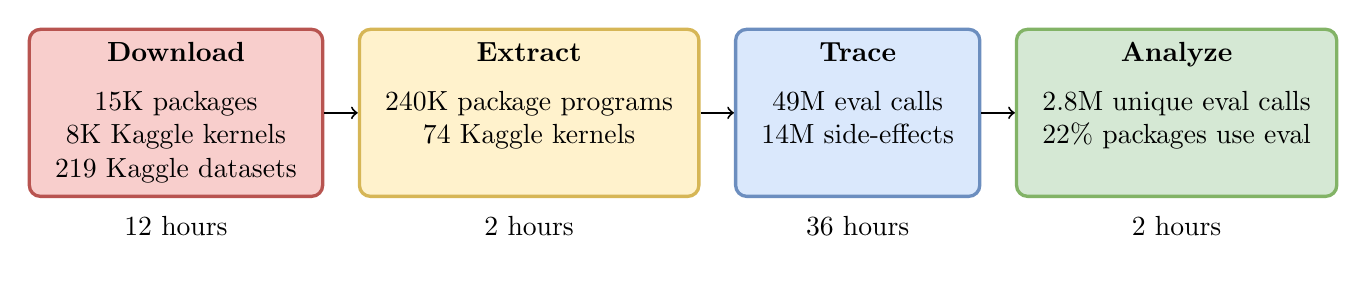
\begin{tikzpicture}
       \definecolor{red}{HTML}{F8CECC}
       \definecolor{darkred}{HTML}{B85450}
       \definecolor{yellow}{HTML}{FFF2CC}
       \definecolor{darkyellow}{HTML}{D6B656}
       \definecolor{blue}{HTML}{DAE8FC}
       \definecolor{darkblue}{HTML}{6C8EBF}
       \definecolor{green}{HTML}{D5E8D4}
       \definecolor{darkgreen}{HTML}{82B366}
       \newcommand{\nodesep}[0]{0.035 \textwidth}
       \newcommand{\textsep}[0]{0.005 \textwidth}
       \newcommand{\nodename}[1]{\begin{tabular}{c}#1\end{tabular}}
       \newcommand{\nodedesc}[1]{\begin{tabular}{c}#1\end{tabular}}
       \tikzstyle{block}     = [rectangle, rounded corners, minimum width=0.15 \textwidth, minimum height=60pt]
       \tikzstyle{connector} = [line width=0.25mm, ->]

       \node [block, fill = red, draw = darkred, very thick] (download) {
         \nodename{
           \vspace{1mm}\textbf{Download}\vspace{1mm}\\
           15K packages\\
           8K Kaggle kernels\\
           219 Kaggle datasets
         }
       };
       \node [below = \textsep of download]   (downloaddesc)   {\nodedesc{12 hours}};
       \node [block, right = \nodesep of download, fill = yellow, draw = darkyellow, very thick] (extract) {
         \nodename{
           \vspace{1mm}\textbf{Extract}\vspace{1mm}\\
           240K package programs\\%, 4.6M LOC\\
           74 Kaggle kernels\\%, 13K LOC\\
           \newline
         }
       };
       \node [below = \textsep of extract]   (extractdesc)   {\nodedesc{2 hours}};
       \node [block, right = \nodesep of extract, fill = blue, draw = darkblue, very thick] (trace) {
         \nodename{
           \vspace{1mm}\textbf{Trace}\vspace{1mm}\\
           49M eval calls \\
           14M side-effects\\
           \newline
         }
       };
       \node [below = \textsep of trace]     (tracedesc)     {\nodedesc{36 hours}};
       \node [block, right = \nodesep of trace, fill = green, draw = darkgreen, very thick] (analyze) {
         \nodename{
           \vspace{1mm}\textbf{Analyze}\vspace{1mm}\\
           2.8M unique eval calls\\
           22\% packages use eval\\
           \newline
         }
       };
       \node [below = \textsep of analyze]    (analyzedesc)    {\nodedesc{2 hours}};
       \draw [connector] (download)   edge (extract);
       \draw [connector] (extract)    edge (trace);
       \draw [connector] (trace)      edge (analyze);
     \end{tikzpicture}
   }
   \caption{Pipeline}\label{fig:pipeline}
 \end{figure}

\begin{compactenum}[(1)]
\item \emph{Download.} Packages are downloaded from CRAN, for Kaggle a web
  crawler retrieves code, and a command-line tool gets data. Installation is
  complicated by native dependencies which sometimes have to be resolved
  manually.
\item \emph{Extract.} The \genthat tool extracts all runnable code snippets and
  turns each of these into a self-standing program~\cite{issta18}, \k{knitr}
  extracts code from notebooks. Each extracted script is instrumented with calls
  to our dynamic analyzer in a way that avoid recording calls to \eval
  originating from our execution harness.
\item \emph{Trace.} Script run with a modified R interpreter to capture calls
  to \eval in CRAN packages. Each script is run in its own process with the GNU
  R compiler turned off to avoid recording its execution.
\item \emph{Analyze.} Analysis outputs are merged, cleaned, and summarized.
  RMarkdown notebooks process the summarized data to generate all graphs (PDF
  from \k{ggplot2}) and numbers (exported as \LaTeX macros) appearing in the
  paper.
\end{compactenum}

\medskip The pipeline runs in parallel~\cite{GNUparallel} orchestrated by a
Makefile. Servers have identical environments thanks to a docker image with all
dependencies installed.

\subsection{Dynamic Analysis}

The tracer that performs dynamic analysis of R scripts is built on top of
\rdyntrace, an extended R 4.0.2 virtual machine that exposes callbacks for
various runtime events~\cite{oopsla19b}. The tracer registers callbacks to all
variants of \eval and a few additional functions to locate the origin of \eval
arguments. It captures dynamic code loading, as well as variable definition and
assignment, allowing us to record side effects that happen in environments
while evaluating code in \eval. A challenge was that lack of source code
references for expression that are not within block surrounded by braces. This
is unfortunately not easily fixed. We extend our dynamic analysis tool to
attach synthetic source code references to all \eval call sites, but the
approach fails in some edge cases. For performance reasons, the tracer is an R
package written in C++ (3.2K LOC) and R (1.3K LOC). While in theory the
implementation should be straightforward, not so in practice. Lazy evaluation
requires delaying the processing of arguments until (and if) they are forced.
Accounting for side-effects performed in an \eval is complicated by the fact
that R is implemented in a mixture of R and C, and that the language
implementation can (and does) call \eval. Lastly, large code bases exercise
many edge cases of the highly underspecified R behavior.

\paragraph{Limitations.} Even with the extension described above, there are
\PkgUndefinedRnd \eval calls without source information (\PkgUndefinedRatio of
all \eval calls). This happen when \eval is an argument to a higher-order
function or when it is called from native code. Another limitation is that we
do not record calls to the native \eval. Neither of these limitations should
invalidate our conclusions.

%%%%%%%%%%%%%%%%%%%%%%%%%%%%%%%%%%%%%%%%%%%%%%%%%%%%%%%%%%%%%%%%%%
\section{Measuring Eval}
%%%%%%%%%%%%%%%%%%%%%%%%%%%%%%%%%%%%%%%%%%%%%%%%%%%%%%%%%%%%%%%%%%

This section reports on the frequency of \eval in CRAN. We use \emph{site} to
refer to an occurrence of a call site to the \eval function in the source code
and \emph{call} to denote an observed invocation of the \eval function.

There are \PkgEvalCallSites \eval sites in \PkgPackages packages;
\PkgPackagesRatio packages use \eval. Over half of these packages have fewer
than 3 sites, and with the exception \MaxEvalCallSitesPackage which has
\MaxEvalCallSitesCount sites, all packages contain fewer than
\MaxEvalCallSitesRest sites. Fig~\ref{fig:pkgs-eval-callsites-hist} shows a
histogram of sites per package. Sites appear in \PkgFunsWithEval functions;
\CranFunsWithEvalRatio of all functions use \eval.

Our pipeline runs \CranRunnableScripts scripts extracted from \CranPackages
packages. Any run that does not call \eval is discarded, leaving us with
\packageNbruns runs. In these runs, \packageAllcalls \eval calls were recorded
originating from \PkgHitEvalCallSites sites. The runs exercised
\PkgHitEvalCallSitesAvgRatio of sites, a ratio similar to the package code
coverage metric which is \PkgCodeCoverage. The reasons some sites are not
exercised can be chalked down to incomplete tests and analysis failures
(\PkgFailedProgramsRatio of the runs crashed or timed out).
Fig.~\ref{fig:traced-eval-callsites} plots exercised site with respect to all
sites for each program; as can be seen coverage is unequal.
Table~\ref{tab:freq} summarizes the frequency of calls, call counts on the left and
number of packages on the right. There are \packageFewcalls packages with fewer
than 100 calls, and \packageManycalls packages with more than 1,000 calls.
\packageMaxcallspack calls \eval \packageMaxcalls times and thus accounts for
over half of our observations.

\begin{figure}[H]
  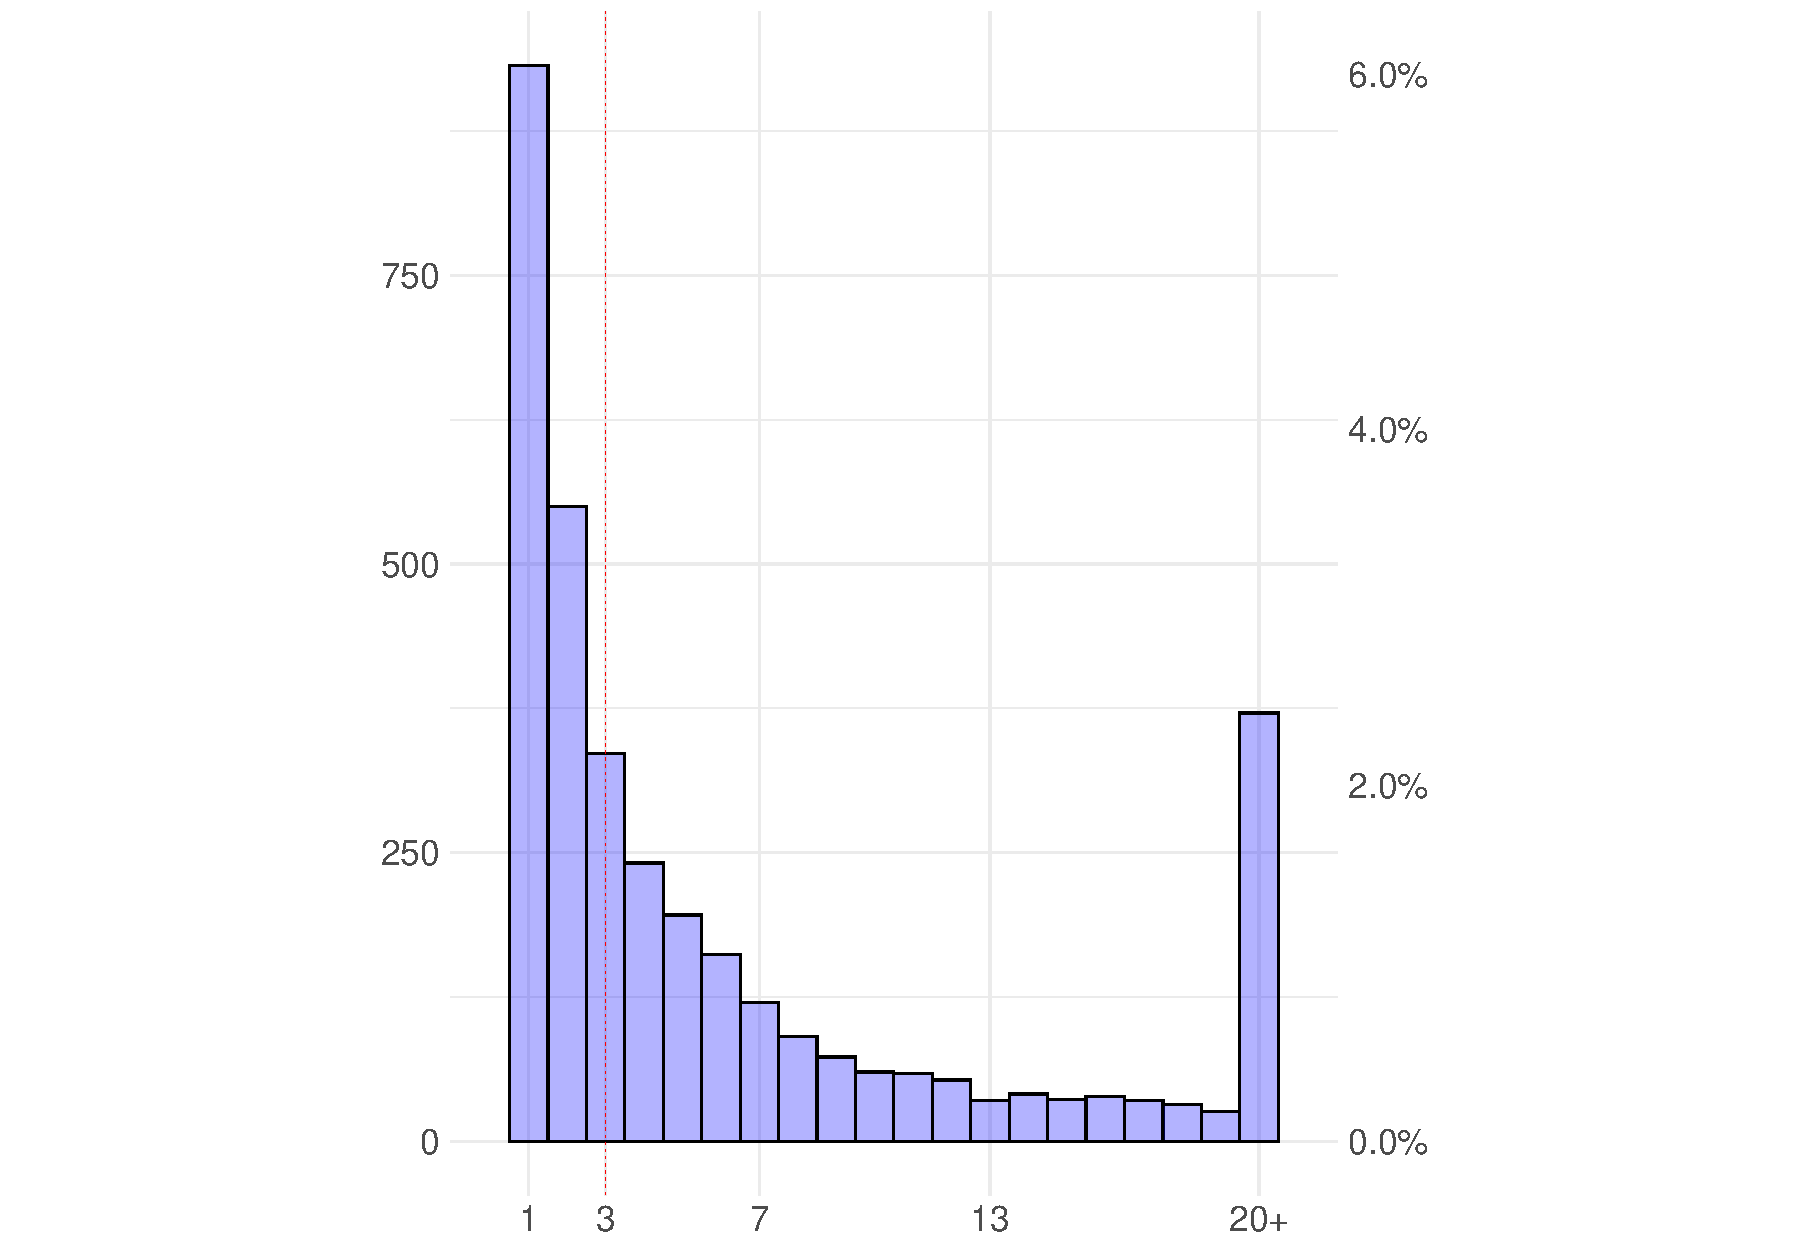
\includegraphics[width=9cm]{pkgs-eval-callsites-hist.pdf}
  \caption{ \eval call sites}\label{fig:pkgs-eval-callsites-hist}
\end{figure}
\begin{table}[H]
\centering
  \small
\begin{tabular}{@{}l@{\hspace{1.5cm}}l@{}}
\begin{minipage} {5cm}\small
  \begin{tabular}{r@{\,}r@{\,}l@{}r|r@{\,}r@{\,}l@{}r} \toprule
    \multicolumn{3}{c}{\bf \small\#calls} &\bf \small \#pck
&     \multicolumn{3}{c}{\bf \small\#calls} &\bf \small\#pck \\\midrule
\tt 1 &--& \tt 10      & \packageBina  & \tt 10K &--&\tt 100K  & \packageBine\\
\tt 11 &--& \tt 100    & \packageBinb  & \tt 100K &--&\tt 1M  & \packageBinf\\
\tt 101 &--& \tt 1K    & \packageBinc  & \tt 1M &--&\tt 10M   & \packageBing\\
\tt 1K &--& \tt 10K    & \packageBind  & \tt 10M &--& \tt 100M & \packageBinh\\\bottomrule
\end{tabular}
\caption{Call frequency}\label{tab:freq}
\end{minipage}
&
\begin{minipage}{7cm}\small
\begin{tabular}{@{\,}r|rrrr}\toprule
  &\eval & \k{evalq} & \k{eval} & \k{local}\\[-1.5mm]
           & & & \k{.parent} &\\\midrule
\small Static sites &\packageStaticeval&\packageStaticevalq&\packageStaticevalparent&\packageStaticlocal \\
\small Exercised sites&\packageTriggeredeval&\packageTriggeredevalq&\packageTriggeredevalparent&\packageTriggeredlocal\\
\small Invocations&\packageEvalsRnd&\packageEvalqsRnd&\packageEparentsRnd&\packageLocalsRnd\\\bottomrule
\end{tabular}~\\[2mm]\caption{Variants}\label{tab:variantseval}
\end{minipage}\end{tabular}

\end{table}
\begin{figure}[H]
  \includegraphics[width=.8\textwidth]{traced-eval-callsites.pdf} \centering
  \caption{\eval call sites coverage of the \PkgPackages packages.}%
  \label{fig:traced-eval-callsites}
\end{figure}

Table~\ref{tab:variantseval} summarizes use of variants, the first row has sites
(\emph{static}), the second has sites encountered during analysis
(\emph{exercised}) and the last gives calls (\emph{invocations}). Most sites and
calls go to \eval itself, \k{eval.parent} is rare, and both \k{evalq} and
\k{local} are barely used at all.

\begin{wraptable}{r}{5cm}  \small  \vspace*{-2mm}\centering
  \begin{tabular}{r@{\,}r@{\,}l@{\,}r|r@{\,}r@{\,}l@{}r} \toprule
    \multicolumn{3}{c}{\bf \#calls} & \bf \#sites &
     \multicolumn{3}{c}{\bf \#calls} & \bf \#sites \\\midrule
    \tt 0 &--& \tt 50    & \packageRunbina & \tt 501 &--& \tt 1000   & \packageRunbine\\
    \tt 51 &--& \tt 100  & \packageRunbinb & \tt 1001 &--& \tt 1500  & \packageRunbinf\\
    \tt 101 &--& \tt 250 & \packageRunbinc & \tt 1501 &--& \tt 2000  & \packageRunbing\\
    \tt 251 &--& \tt 500 & \packageRunbind & \tt 2001 &--& \tt 3000 & \packageRunbinh\\\bottomrule
  \end{tabular}
  \caption{Normalized calls} \label{tab:cn}
\end{wraptable}

Table~\ref{tab:cn} shows average count of calls from a given site and given run and
how many sites fall in that range. For instance, \packageRunbinh sites are
called over 2,000 times per run. Larger call counts suggest the presence of
loops or recursive functions, but given the data this seems to be the exception;
\packageRunbina of sites are called fewer than 50 times, most sites are invoked
once and half as many are invoked twice.

\Eval accepts any value as argument, but if the value is not an expression,
\eval returns it unchanged. Expressions account for \packageCodepercent of
arguments. More specifically, \packageSymbolpercent are symbols (variables
such as \k{x}), \packageLanguagepercent are language objects (expressions
representing a function calls), and \packageExpressionpercent are expression
objects (lists of expressions). Further inspection reveals that \k{\_inherit}
accounts for \packageGgplotsymbolpercent of symbols and comes from one site in
\k{ggplot2}.\footnote{Each object has a field model inheritance, this comes from
\k{ggproto}, one of the many object-oriented systems for R.}


\begin{wrapfigure}{r}{6.2cm}
\begin{tabular}{c}
{\hspace{-25mm}\includegraphics[width=0.8\textwidth]{package_size_loaded_distribution}}
\end{tabular}
\caption{Loaded code} \label{fig:sizedistribution}
\end{wrapfigure}

To estimate how much executable code is injected through \eval, we measure the
size of the arguments in terms of number of nodes. For example,
\k{expression(x+1)} has a size of 3. The large number of symbols skew the median
to \packageMedianszeval but the average size is \packageAvgszeval nodes. The
largest \eval input we observed was an expression of \packageMaxszeval nodes, a
significant chunk of code. Fig.~\ref{fig:sizedistribution} shows the
distribution of sizes for arguments of fewer than 25 nodes. Sizes drop rapidly,
there are few observations larger than 15 nodes. The long tail is omitted for
legibility. As an alternative to counting nodes, we tried measuring string
lengths of expressions after calling a function to deparse values back to
strings, but these measurements were dominated by massive data objects which
could range in the MBs.

To assess how much computational work is performed in \evals, we count the
instructions executed by the interpreter. Most call do relatively little, with
\packageSmalleventspct of calls executing fewer than 50 instructions. The violin
plot of Fig.~\ref{ev}(a) shows the distribution of short running \evals; the
data is dominated by \evals which simply perform symbol lookup. Fig.~\ref{ev}(b)
shows the distribution of work-intensive \evals which go all the way to
\packageMaxeventsRnd instructions.

\begin{figure}[h!]
\begin{tabular}{@{}c@{}c@{}}
\begin{minipage}{7.5cm}
 \includegraphics[width=\textwidth]{package_events_per_pack_small}
\end{minipage}&\begin{minipage}{7.5cm}
  \includegraphics[width=\textwidth]{package_events_per_pack_large}
\end{minipage}\\[-3mm]
\small (a) Small & \small (b) Large
\end{tabular}
 \caption{Instructions per call} \label{ev}
\end{figure}

\paragraph{Discussion.}
\Eval is widely used in CRAN packages. Nearly every fourth package contains at
least one \eval call site. However, most packages use \eval modestly. Packages
that rely heavily on \eval are mostly ones that provide statistical modeling and
simulation functions. At runtime, over a third of our scripts triggered calls to
\eval, note that all scripts performed \eval originating from base package but
these are disregarded here. Half of the calls come from a single site, for the
rest, most packages have low call frequency. The data is consistent with usage
of \eval for configuration and meta-programming and not in performance sensitive
contexts such as loops. While most arguments to \eval are small, often just a
variable name, and do little work, we have also observed large \eval arguments
and arguments that perform massive amounts of work.

%%%%%%%%%%%%%%%%%%%%%%%%%%%%%%%%%%%%%%%%%%%%%%%%%%%%%%%%%%%%%%%%%%%%%%%%%
%%%%%%%%%%%%%%%%%%%%%%%%%%%%%%%%%%%%%%%%%%%%%%%%%%%%%%%%%%%%%%%%%%%%%%%%%
\section{A Taxonomy of \Eval}

The previous section gave a quantitative view of \eval usage; we now try to
elucidate \emph{what} it does.

\subsection{The expression in \eval} \label{sec:minimized}

\begin{table}[!b]\small
\hspace*{-0.2cm}
\begin{tabular}{crrrrrc}\toprule
  \bf $min(e)$& \bf \#sites & \bf \%sites & \bf \#packages & \bf \#ops & \bf \%envir & \bf example\\\midrule
\k{X}&\packageMinimizedcallsitesa &\packageMinimizedpropsitesa &\packageMinimizedpackagea &\packageMinimizedmedianoperationsaRnd &\packageMinimizedpercentparentframesa & \k{y+1}\\
\k{F(F(X))} & \packageMinimizedcallsitesb  & \packageMinimizedpropsitesb & \packageMinimizedpackageb  & \packageMinimizedmedianoperationsbRnd & \packageMinimizedpercentparentframesb & \k{gbov( mean(x), a-1)}\\
\k{V}&\packageMinimizedcallsitesc &\packageMinimizedpropsitesc &\packageMinimizedpackagec &\packageMinimizedmedianoperationscRnd &\packageMinimizedpercentparentframesc& \k{c(42,21,0)}\\
\k{F(X)}& \packageMinimizedcallsitesd & \packageMinimizedpropsitesd & \packageMinimizedpackaged & \packageMinimizedmedianoperationsdRnd & \packageMinimizedpercentparentframesd & \k{seq\_len(iters)} \\
\k{\$} & \packageMinimizedcallsitese & \packageMinimizedpropsitese & \packageMinimizedpackagee & \packageMinimizedmedianoperationseRnd & \packageMinimizedpercentparentframese & \k{DF\$B}\\
\k{model.frame}& \packageMinimizedcallsitesf & \packageMinimizedpropsitesf & \packageMinimizedpackagef & \packageMinimizedmedianoperationsfRnd & \packageMinimizedpercentparentframesf &  \k{model.frame(formula = Z ~ U)}   \\
\k{F()}& \packageMinimizedcallsitesg & \packageMinimizedpropsitesg & \packageMinimizedpackageg & \packageMinimizedmedianoperationsgRnd & \packageMinimizedpercentparentframesg & \k{rgamma(3, 2, n = 10L)} \\
\k{FUN} & \packageMinimizedcallsitesh & \packageMinimizedpropsitesh & \packageMinimizedpackageh & \packageMinimizedmedianoperationshRnd & \packageMinimizedpercentparentframesh & \k{function(x, y) x + 3 * y} \\
\k{<-} & \packageMinimizedcallsitesi  & \packageMinimizedpropsitesi & \packageMinimizedpackagei & \packageMinimizedmedianoperationsiRnd & \packageMinimizedpercentparentframesi & \k{x[1, 2:3, 2:3] <- value}\\
\k{BLOCK} & \packageMinimizedcallsitesj & \packageMinimizedpropsitesj & \packageMinimizedpackagej & \packageMinimizedmedianoperationsjRnd & \packageMinimizedpercentparentframesj & \k{\{write.csv(iris,tf);file.size(tf)\}} \\\bottomrule
\end{tabular}
\caption{Minimized expressions} \label{tab:minimizedexpressions}
\end{table}


The expressions passed to \eval vary widely. We categorize expressions using a
minimization function which abstract some of the incidental details of
expressions and return a ``shape'' that can be used to group similar \evals. The
function $min(e)$ which for a given expression $e$ returns a normal form. Normal
forms use \k{V} to stand in for values occurring in expression, \k{X} stands in
for variables, and \k{F} stands for functions. The function performs constant
folding of arithmetic and string expressions over base operators, for instance
$min(\c{1+1})$ simplifies to $\c{V}$, on the ground that addition of values
likely returns a value. Value simplification takes $min(\c{c(1,2,3+2)})$ to
$\c{V}$ as a complex vector containing values is a value. Variable absorption
has $min(\c{x+y})$ becomes $\c{X}$, this motivated by the fact that addition is
not an ``interesting'' operation, and that \k{X} stands in for any number of
variable lookups. Function absorption simplifies nested functions to keep an
abstraction of the nesting $min(\c{g(f(x),h(z))})=\c{F(F(X))}$. There are other
simplifications, the full list can be found in our artifact. It is worth
mentioning that these simplifications are heuristics, in R \k{1+1} is not
necessary \k{2}. The addition operator can be redefined, but it typically isn't
or at least not in a way that would invalidate arithmetic.

Table~\ref{tab:minimizedexpressions} gives the 10 most frequent shapes with the
number and ratio of sites that received arguments of that shape. Operations is
the median count of instructions performed by the interpreter when evaluating
argument of the given shape. Envir is the ratio of sites that evaluate in a
function environment. The last column has a sample expression that normalizes to
the corresponding shape. We detail these shapes and discuss their implication for
the behavior of \eval.

\newcommand{\EE}[1]{{{\emph{\framebox{#1}}}}\\[1mm]}

\begin{tabular}{@{}p{.97\linewidth}}
  \medskip\EE{$min(e)=\c{V}$}\\[-2mm]\small Values occur in 16\% of sites, 74\% of
  those are constants such as integers, the remainder evaluate to a value (\packageNbCallSitesUniqueActualValue of
  sites only ever see a value). \Eval
  is needed when the expression denoting the values is constructed
  programmatically. Cases when a value is directly given to \eval, and \eval
  returns it unchanged, often occur when a computation has a default path and
  another, more interesting, path that requires evaluation.
  This shape usually run in few interpreter steps.
  The environment in which they evaluate is mostly irrelevant.
\\
\medskip\EE{$min(e)=\c{X}$}\\[-2mm]\small Variable lookups are the most common shape,
\packageNbSymbolVarSitePercent are simple variable names, e.g. \k{x}. The shapes
subsumes \k{V} and built-in arithmetic operations, so a mixture of arithmetics
and variables normalize to \k{X}. A lookup is one step of execution, if a promise
is returned an arbitrary number of additional steps may be needed; the median is
\packageMinimizedmedianoperationsaRnd, suggesting that most variable read do
little work. Variables are often evaluated in environments that have been
constructed programmatically, \packageMinimizedpercentparentframesa of
expressions are evaluated in a function environment.
\\
\medskip\EE{$min(e)=\c{\$}$}\\[-2mm]\small This shape extends \k{X} to include lookup
with the dollar operator, \eg~\k{x\$f}, and vector indexing, \eg~\k{x[42]} and
\k{x[[24]]}. This takes a few more step of evaluation on average, and is
typically used in a function environment.
\\
\medskip\EE{$min(e)=$~\k{<-}}\\[-2mm]\small This includes both direct assignment {\tt
  <-} and parent environment assignment {\tt <\,\!<-} as well as the \k{assign}
function. It subsumes \k{\$}. Assignments represent the most obvious source
of side effects in \eval. Most cases originate from trivial code generation
where the assign expression is assembled using parse or substitute, often in
a loop.
\\
\medskip\EE{$min(e)=\c{F()}$}\\[-2mm]\small Function calls without variable lookups or
assignment. A variable is allowed the function position, looking up
functions does not trigger computation unless the function's name
is bound to a promise. This shape typically does not perform much work.
\\
\medskip\framebox{$min(e)=\c{F(X)}$}~\EE{$min(e)=\c{F(F(X))}$}\\[-2mm]\small Function
calls whose arguments may include variable references and nested calls. Together
they represent the most frequent shape and perform over 16 steps. They are
frequently evaluated in function environments.
\\
\medskip\EE{$min(e)=\c{FUN}$}\\[-2mm]\small Function definitions without any
computation, \eg~\k{function(x) x+1}. In addition to \k{FUN},
\packageGeneralizedFunctionDefinitionSitesPercent of sites have function
definitions nested in other expressions.
\end{tabular}

\begin{tabular}{@{}p{.97\linewidth}}
\medskip\EE{$min(e)=\c{BLOCK}$}\\[-2mm]\small Multi-statement code blocks, as
they can be large we do not try to normalize their contents. They execute in a
median \packageMinimizedmedianoperationsjRnd steps, usually, in function
environments.
Essentially, the block denotes a fragment of a program to be evaluated in a
particular way and in a particular environment. The latter is what makes it
different from 0-argument closure. There is a number of use cases: unit testing
frameworks (\eg \k{testthat}, \k{testit}), code benchmarking (\eg
\k{rbenchmark}, \k{microbenchmark}), running code in parallel (\eg \k{foreach},
\k{doParallel}), or deferring code execution (\eg \k{withr}).
\\
\medskip\EE{$min(e)=\c{model.frame}$}\\[-2mm]\small The \k{model.frame} function
returns a dataframe resulting from fitting the model described in a formula.
This shape subsumes \k{F(F(X))}, \k{FUN}, and assignments. It is the single most
popular function invoked from \eval. Each call does a median of 2K instructions.
\end{tabular}

\paragraph{Discussion.} The number of different shapes that any given
\eval site sees is an indication of the versatility of that site.
\packageNbOneMinimizedPercent of sites only see a single expression shape. It
would be encouraging if one could, given a small training set, predict the shape
of \evals to come. In our corpus, only a few sites are highly polymorphic with
more than eight shapes. An example of those is the pipe operator of the
\k{magrittr} package which is used to compose functions, \eg instead of
\k{f(g(h(x),y),z)} one can write \k{h(x) \%>\% g(y) \%>\% f(z)}. As there many
different patterns of use, there are also many different shapes. In comparison
with R, JavaScript's \eval usage was more straightforward and more predictable
as reported by \citet{oopsla12b}, with 98\% of sites with only one shape. On the
other hand, there are \packageNbSimpleMinimizedOne sites that only receive one
of the simple shape (\ie\xspace \k{X}, \k{V}, \k{\$} or \k{<-}), and
\packageNbSimpleMinimizedMore sites get multiple simple shapes. Among these
sites, there are many cases where \eval could be possibly replaced by simpler constructs
such as \k{get} to lookup a name in an environment, \k{assign} to set a value to
a name in an environment, or \k{do.call} to call a function reflectively.

\subsection{The environments of \eval}\label{sec:env}

Contrary to JavaScript, in R the environment of \eval can be specifies by its
\k{env} argument. This gives users control over what is visible to the
computation started by \eval and the potential reach of its side-effects. We
distinguish the following kinds of environments:

\begin{itemize}[---]
\item \emph{Function:} environments for the local variables of some function
  currently active on the call stack. Obtained by calling \k{parent.frame()} or
  \k{sys.frame()}.
\item \emph{Synthetic:} environments built from data structures such as lists,
  data.frames, or constructed explicitly with \k{new.env}, \k{list2env}, or
  \k{as.environment} or the empty environment.
\item \emph{Global:} environments in which scripts or interactive commands are
  evaluated.
\item \emph{Package:} environments of libraries.
\end{itemize}


Table~\ref{tab:highlevelenvironments} shows that most calls evaluate in the
scope of a function, global is a distant second. This means that most reads and
writes act on local variables. But of which function? Table~\ref{tab:funoffset}
gives the offset of that function on the call stack: 0 is the function that called
\eval, 1 is that function's caller, and so on. In 81\% of cases, \eval uses
its caller's environment -- the variables of the function where the call to \eval
textually occurs are read and written. About 1.5\% of sites evaluate their
argument three frames up the call stack, or above. Modular reasoning is thus
impossible in R. Since the actions of \eval happen at a distance, understanding
any given code snippet requires knowing which functions may be called
transitively from that snippet. In \packageNbOneCategoryEnvirSitePercent of
the sites, only one kind of environment is observed.

\begin{table}[h]
  \centering\small\hspace{-.5cm}
\begin{minipage}{3.7cm}
  \begin{tabular}{@{}rrr@{}}\toprule
 \bf Kind & \bf \#sites & \bf \%sites \\\midrule
 Function & \packageNbFunctionEnvSites &  \packageNbFunctionEnvSitePercent\\
 Synthetic & \packageNbSyntheticEnvSites & \packageNbSyntheticEnvSitePercent \\
 Global &  \packageNbStrictGlobalEnvSites & \packageNbStrictGlobalEnvSitePercent \\
 Package & \packageNbPackageNamespaceEnvSites & \packageNbPackageNamespaceEnvSitePercent \\\bottomrule
\end{tabular}
\caption{Kinds per site} \label{tab:highlevelenvironments}
\end{minipage}\hspace{-.2cm}
\begin{minipage}{3.7cm}\centering
  \begin{tabular}{@{}rrr@{}}\toprule
 \bf Offset & \bf \#sites & \bf \%sites \\\midrule
  \packageCallerEnvHierarchyNamea & \packageCallerEnvHierarchySitesaRnd & \packageCallerEnvHierarchySitePercenta \\
  \packageCallerEnvHierarchyNameb& \packageCallerEnvHierarchySitesbRnd & \packageCallerEnvHierarchySitePercentb \\
  \packageCallerEnvHierarchyNamec& \packageCallerEnvHierarchySitescRnd & \packageCallerEnvHierarchySitePercentc  \\
$\ge 3$& \packageNbFarAwayCallerSites &  \packageNbFarAwayCallerSitePercent \\\bottomrule
 \end{tabular}
\caption{Function offset}\label{tab:funoffset}
\end{minipage}\hspace{-.2cm}
\begin{minipage}{3.7cm}
  \begin{tabular}{@{}rrr@{}} \toprule
\bf Parent & \bf \#sites & \bf \%sites \\\midrule
Function & \packageNewEnvCategorySitesa & \packageNewEnvCategorySitePercenta \\
Package & \packageNewEnvCategorySitesb &  \packageNewEnvCategorySitePercentb\\
Global & \packageNewEnvCategorySitesc & \packageNewEnvCategorySitePercentc \\
    Empty & \packageNewEnvCategorySitesd & \packageNewEnvCategorySitePercentd \\\bottomrule
\end{tabular}
\caption{Wrapper envs.} \label{tab:newenvs}
\end{minipage}\hspace{-.2cm}
\begin{minipage}{3.7cm}\centering
  \begin{tabular}{@{}ccc@{}} \toprule
 \bf \#kinds & \bf \#sites &  \bf \%sites \\\midrule
 \packageNbCategoryEnvira & \packageNbCategoryEnvirSitesaRnd &  \packageNbCategoryEnvirPercenta\\
 \packageNbCategoryEnvirb &  \packageNbCategoryEnvirSitesbRnd & \packageNbCategoryEnvirPercentb \\
 \packageNbCategoryEnvirc & \packageNbCategoryEnvirSitescRnd &  \packageNbCategoryEnvirPercentc\\
 \packageNbCategoryEnvird & \packageNbCategoryEnvirSitesdRnd & \packageNbCategoryEnvirPercentd\\\bottomrule
\end{tabular}\caption{Multiplicities}\label{tab:polyenvir}
\end{minipage}\hspace{-1cm}
\end{table}

Each synthetic environment has a parent that is specified when calling
\k{new.env}. When \k{envir} is a list or a data frame, \eval uses its third
argument (\k{enclos}). The parent is used to search for variables not found in
its child (side-effects stay in the child). Table~\ref{tab:newenvs} shows parent
kinds for synthetic environments. Most of them are functions.

Global \evals split between intentional and accidental one. Direct references to
the top-level, using \k{globalenv()} or \k{.GlobalEnv}, are rare; they occur in
only \packageNbExplicitGlobalSites sites. Thus we suspect most uses of global
are accidental. They arise from the fact that our corpus consists of many code
snippets that are run at the top-level, global is thus the caller of \eval. This is
noteworthy because writes to global variables are visible to all functions and
are not reclaimed by the garbage collector. So accidental uses may pollute that
namespace. Table~\ref{tab:polyenvir} gives the number of kinds seen at a given
call site.

\paragraph{Discussion.}
The data presented here is not surprising. The main use of \eval is to provide a
customizable extension mechanism for the behavior of functions. They are a way
to parameterize the function with any behavior that can be expressed in R. The
behavior of \eval within its enclosing function is to read and write variables,
mostly read, and very rarely, delete variables. There are also some cases where
new variables are injected in a function. Usually, this in the direct caller,
but it can sometimes take effect several frames up the call stack. There is
something brittle about code relying on the position of a caller, a lot of
refactoring may break code that does that.

One bit of information that we lack is how the environment was obtained. Our
expectation is that the expression was extracted from a promise using
\k{substitute}, perhaps modified, and then evaluated with the environment coming
from the same promise. We believe the case where \eval is provided with the results
of programmatically selecting some call stack to be less frequent.

Synthetic environments are relatively frequent. Common uses-case include
evaluation of an expression in a sandbox, or using a data structure as
environment. For example one could evaluate a method of an object and use an
environment to hold the object's fields.

We have already explained the popularity of global environments. As for package
environments, they are used in only \packageNbPackageNamespaceEnvSites sites.
This is probably for the best as mutating the bindings of a loaded package is
frowned upon and R tries to discourage it.

\subsection{The origins of \eval}

Where does the expression passed to \eval come from? There are various means of
creating an expression, often these means correlate with a particular use case.
Our analysis records the values returned by some functions of interest as well
as their arguments. We build a direct acyclic graph that track the origin
of the values that are given to \eval. Fig~\ref{fig:provgraph} shows an example
of the origin graph for the expression \k{e}.
The origin of \k{e} includes both \k{parse} and \k{quote}. We pick an
origin by traversing the graph from the terminal leaf, \ie from the \eval node, following the left-hand side
member of assignments until reaching a root node. It represents the origin that is
further modified to yield the expression passed to \eval. In our example, the
origin is \k{parse}.

\begin{figure}[H]
  \begin{minipage}{.39\textwidth}
    \vspace{-5mm}
\begin{lstlisting}
 > e <- parse(text = "a;b")
 > e[[2]] <- quote(c) # e is a;c
 > eval(e)
\end{lstlisting}
  \end{minipage} \hspace{2cm}
 \begin{minipage}{.4\textwidth}
	\centering\scalebox{.7}{
	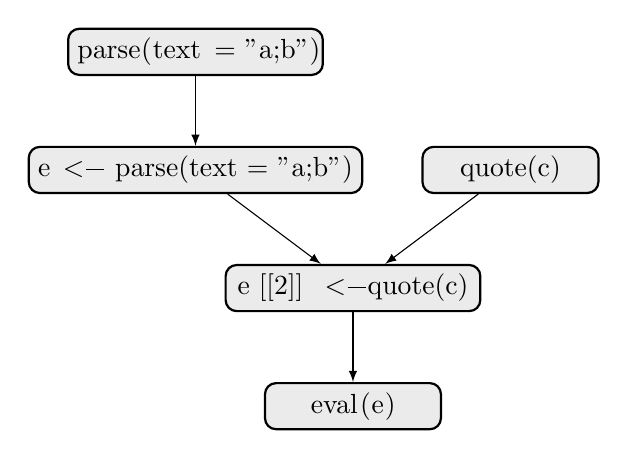
\begin{tikzpicture}[
		every node/.style={draw, rounded corners, fill=LightGray, text width = 2cm, align = center, thick}
		]
		\node (E) at (2,0) {\k{eval(e)}};
		\node[text width = 3cm] (CA) at (2, 1.5) {\k{e[[2]] <-quote(c)}};
		\node (Q) at (4, 3) {\k{quote(c)}};
		\node[text width = 4cm] (A) at (0, 3) {\k{e <- parse(text = "a;b")}};
		\node[text width = 3cm] (P) at (0, 4.5) {\k{parse(text = "a;b")}};

		\draw[<-, >=latex] (E) -- (CA);
		\draw[<-, >=latex] (CA) -- (Q);
		\draw[<-, >=latex] (CA) -- (A);
		\draw[<-, >=latex] (A) -- (P);
	\end{tikzpicture}}
\end{minipage}
\caption{Example of an origin graph} \label{fig:provgraph}
\end{figure}


% Wrap tables do not play well with lists (they warn about it in the documentation actually!)
\begin{wraptable}{r}{5cm}\small\centering
\begin{tabular}{lcc}\toprule
\bf Provenance & \bf \#sites & \bf \%sites \\\midrule
		\packageProvenanceNamea & \packageNbProvenanceSitesa & \packagePercentProvenanceSitesa \\
		\packageProvenanceNameb & \packageNbProvenanceSitesb & \packagePercentProvenanceSitesb \\
		\packageProvenanceNamec & \packageNbProvenanceSitesc & \packagePercentProvenanceSitesc \\
		\packageProvenanceNamee & \packageNbProvenanceSitese & \packagePercentProvenanceSitese \\
		\packageProvenanceNamef & \packageNbProvenanceSitesf & \packagePercentProvenanceSitesf \\
		\packageProvenanceNameg & \packageNbProvenanceSitesg & \packagePercentProvenanceSitesg \\
		\packageProvenanceNameh & \packageNbProvenanceSitesh & \packagePercentProvenanceSitesh \\
		\packageProvenanceNamei & \packageNbProvenanceSitesi & \packagePercentProvenanceSitesi \\
		\packageProvenanceNamel & \packageNbProvenanceSitesl & \packagePercentProvenanceSitesl \\
		\packageProvenanceNamen & \packageNbProvenanceSitesn & \packagePercentProvenanceSitesn \\\bottomrule
\end{tabular}

\medskip

\begin{tabular}{rrr} \toprule
\bf Origin  & \bf \#sites & \bf \%sites \\\midrule
Reflection &  \packageNbReflectionSites & \packageReflectionSitesPercent\\
String & \packageNbStringSites & \packageStringSitesPercent \\
Constructed & \packageNbConstructedSites & \packageConstructedSitesPercent \\
Environment & \packageNbSymbolSites & \packageSymbolSitesPercent \\
External & \packageNbExternalSites & \packageExternalSitesPercent \\\bottomrule
\end{tabular}
\caption{Origins}\label{tab:provenance}\vspace{-1cm}
\end{wraptable}

To have a high-level views of provenance we classify functions into the
following five categories:

\begin{itemize}[---]
\item {\it Reflection:} use of \k{match.call} to reflectively capture the
  expression that invoked this function, arguments are promises, and
  \k{substitute} is used to retrieve their source.
\item {\it String:} create from strings by invoking \k{parse},
  \k{str2lang}, or \k{str2expression}.
\item {\it Constructed:} invoked \k{quote} or \k{expression}, or by built with
  \k{call} or \k{as.call}.
\item {\it Environment: } created with \k{as.name} or \k{as.symbol}, typically
  to read a non-local environment.
\item {\it External: }  call to a C function. % Put an example
\end{itemize}

Table~\ref{tab:provenance} summarizes origins. Is shows frequencies by function
and by category. For technical reasons, we misclassify a small number of sites.
Manual inspection of numerous examples suggests that errors are rare. Some sites
are counted multiple times as they are invoked with different origins. Strings
correlate with dynamic code loading as done by \k{source} and \k{sys.source}.
Few calls (\packageNbParseFromFileSites in total) consume the result of calling
\k{parse} on a file. Most build strings programmatically.


\paragraph{Discussion}
The main use cases for \eval involve using \k{match.call}, \k{substitute}, or
\k{formals} to access and transform arguments of a function. Constructing
expressions from strings is also a common use case. The constructed category
shows that most \evals come from existing code that was modified by the
programmer before invoking \eval. Both constructed and reflection categories
roughly correspond to meta-programming. Some uses could be replaced by
macros if the R designers could be convinced to overcome their distaste for
those.

\subsection{The effects of \eval}

\Eval may perform side-effects. We care about effects that are visible after a
call finishes, \ie variable definitions, updates, and removals. Knowing in which
environments these side-effects happen, can help determine the impact of \eval
on our ability to reason about the code. Our analysis records information about
every environment. From the recorded data, we discard side-effects coming from
unit testing frameworks as they use \eval to run all their tests and thus
dominate the side-effect data.\footnote{The corpus has \k{RUnit, testthat,
  tinytest} and \k{unitizer} testing frameworks.}

We record \SEAllRnd side-effects from \SEAllCallsRnd calls and \SEAllSites
sites. The challenge is to remove accidental side-effects caused by the R
virtual machine implementation and not user code. For example, the
\k{.Random.seed} variable is saved and restored from and to the global
environment every time a statistical routine is called. Filtering out accidental
side-effects leaves us with \SEUserRnd writes from \SEUserCallsRnd calls (in
\SEUserSites sites and \SEUserFunctions functions). In this set, \SEFunsNighty functions are
responsible for 90\% of side effects. Half of those come from just three
functions: \k{plyr::allocate\_column} (allocates space for a new data frame
column), \k{withr::execute\_handlers} (executes deferred expressions), and
\k{foreach::doSEQ} (executes an expression on each element in a collection,
possibly in parallel). Most of the sites (\SESitesInEnvirRatio) update
the environment specified by the \k{env} parameter.

\begin{table}[!h]
  \begin{tabular}{lrrrr}
    \toprule
    \bf Environments & \bf \#sites & \bf \%sites & \bf \#funs. & \bf \%funs. \\%
    \midrule
    \expandableinput tag/table-se-target-envs.tex
    \bottomrule
  \end{tabular}
  \caption{Target environments for side-effects} \label{tab:se-env}
\end{table}

Table~\ref{tab:se-env} shows environment kinds where side-effects happen.
Function environments distinguish between \emph{local}, the caller environment
(offset 0), and \emph{function} (offset >0). \emph{Synthetic} represents
constructed environments. \emph{Object} is used to denote the environments
attached to objects and classes in the S4 and R6 object systems. \emph{Multiple}
denotes cases where side-effects to more than one kind originate from one site.
The table gives the number of call sites of \eval (and the ratio) performing
side-effect in a particular environment kind. The table also gives the number of
functions in which these sites occur (and ratio).

Most sites, \SESitesInOneClass, do all their side-effects consistently in one
kind of environments. The same happens at the function level. Almost half of the
sites (over a third of the functions) do side effects in either \emph{Local} or
\emph{Object} environments.

Table~\ref{tab:se-types} shows recorded effects. There are over 5M updates. In
terms of calls, we see assignments primarily and in terms of site definitions.
This is expected. A subsequent \eval call will turn a definition into an update.
The most dangerous side effect is variable removal, as it means that after a
call to \eval some binding in some environments will disappear. While rare, this
happens, but the vast majority comes from a single site
(\k{withr::execute\_handlers}). This makes sense as it is used to defer
evaluation of an expression to after the function exit and thus used for clean
up. It is used almost exclusively by the \k{tidyselect} package for removing the
reference to the current quosure environment while interpreting a data frame
column selectors.\footnote{\cf \url{https://tidyselect.r-lib.org/}}

Looking closely at the value types in variable updates, we observe that the
majority of \eval sites involve basic R vectors (\SEBasicTypeRatio) and lists
(\SEListTypeRatio). From the compiler perspective, we would like to know how
many sites change function bindings. In the corpus, this happens in only
\SEClosureType sites; \SEClosureTypeLocal of them do that in the local
environment. We have manually inspected a few of these sites, but except for
manual injection of parameters into a \k{model.frame} execution environment, we
did not find a common use case.

\begin{table}[h]
  \small
  \centering
  \begin{tabular}{lrrrrrr}
    \toprule
    \bf Side effect & \bf \#events & \bf \%events & \bf \#calls & \bf \%calls & \bf \#sites & \bf \%sites \\%
    \midrule
    \expandableinput tag/table-se-types.tex
    \bottomrule
  \end{tabular}
  \caption{Types of \eval side-effects} \label{tab:se-types}
\end{table}

Out of the minimized expressions, it is \k{BLOCK}, \k{<-} and \k{F(F(X))} that
contribute to the vast majority of side effects. Concretely, 92\% of \k{BLOCK},
87\% of \k{<-} and 15\% of \k{F(F(X))} expressions do side effects. In the case
of \k{BLOCK}, most of them happen in the environment passed to the \eval call
(default is the parent environment). For \k{<-} it is 15\%. However, this form
is dominated by the \k{plyr::allocate\_column} function that side-effects in
the environment containing the data frame to which it allocates new column.
Without this call, \k{<-} is similarly predictable with 96\% of side effects
happening in the passed environment. For \k{F(F(X))}, it is less clear as 58\%
of side effects happen in a different environment to the one that was passed to
\eval.

\paragraph{Discussion} In JavaScript assignments in \eval can happen in either
local scope or less often, when called through an alias, in the global scope.
In R, given the support for first-class environments, it can happen anywhere,
making it \eval more dangerous than it already is. However, the data suggest
that first, side-effects from \eval are not as widespread as in the case of
JavaScript,\footnote{\citep{ecoop11} shows that in the \emph{Interactive}
  scenario, \eval in Javascript performs, store events can reach up to 40\% of
the events, and 7\% to 8\% of the \eval do side effects in the global scope. }
and that over half of them happen in a predictable environment. This gives a
ray of hope for a hypothetical R compiler. Even though \eval can do anything
anywhere, the data suggests most effects are sane.

\section{Usage of \eval}

The R language was intended to be extensible. The combination of lazy
evaluation, \k{substitute} and \k{eval} are some of the tools given to
developers to this end. To understand \emph{why} developers use \eval, we
manually inspected top 117 sites which contribute to 90\% of the calls in the
corpus. This section gives some real-world examples, we simplify code for
clarity.

\paragraph{Extended Interfaces}
Sometimes it is convenient to allow users to extend the behavior of a library
function. \Eval allows clients to provide a simple text string that shall be
executed in the context of the function. The example here allows users to
provide formulas as strings, such as \k{"exp(-x^2/2)"}, the contract being that
the text can refer to some variable \k{x} that will be set up by the called
function. In this case one users could provide an anonymous function.

\begin{minipage}{.95\textwidth}
\medskip\underline{\c{AdapSamp::rARS}:}
\begin{lstlisting}
 function(n,formula) {
    p <- function(x) eval(parse(text=formula))
\end{lstlisting}\medskip
\end{minipage}

\paragraph{Code Generation}
\Eval can be used to generate boiler plate code that would either be tedious to
write by hand or that is only known after deployment. The example uses \eval to
automatically generate R bindings to C++ methods.

\begin{minipage}{.95\textwidth}
\medskip\underline{\c{Rcpp::.makeCppMethods}:}
\begin{lstlisting}
 function(methods,env) {
   for(what in cppMethods)
     methods[[what]] <-
       eval(substitute(function(...)CppObject$what(...)), env)
\end{lstlisting}\medskip
\end{minipage}

\paragraph{Extracting Varargs}
A somewhat odd use of \eval is to obtain the source code of the arguments passed
to a vararg parameter. In this example, the function iterates over the contents
of the vararg until it finds a non-null value. \k{substitute(alist(...))} yields
an expression that represents a call to \k{alist} but where the \k{...} are
expended with the arguments supplied to the function. \Eval then returns a
\k{list} with unevaluated argument expressions which are evaluated sequentially
for their result.

\begin{minipage}{.95\textwidth}
\medskip\underline{\c{statnet.common::NVL}:}
\begin{lstlisting}
 function(...) {
   for(e in eval(substitute(alist(...)))) {
     x <- eval(e, parent.frame())
     if(!is.null(x)) break
   }
   x
 }
\end{lstlisting}\medskip
\end{minipage}


\paragraph{Controlled Evaluation}
Developer often want to control when and if expressions are evaluated. For
example, a package that provides users with the ability to make assertions and,
if they fail, produce legible error messages. The example here accepts a vararg
with a list of expressions whose code is extracted using
\k{eval(substitute(alist(...)))}. The expression are evaluated sequentially
in the caller's environment. If an expression is false, an error message is
generated.

\begin{minipage}{.95\textwidth}
  \medskip\underline{\c {assertthat::see\_if}:}
\begin{lstlisting}
 function(..., env=parent.frame(), msg=NULL) {
    asserts <- eval(substitute(alist(...)))
    for (assertion in asserts) {
      res <- tryCatch({
        eval(assertion, env)
      }, assertError=function(e) { structure(FALSE, msg=e$message) })
\end{lstlisting}\medskip
\end{minipage}

\paragraph{Shadowing}
%%% TODO ?????????????////
Many packages use \eval to implement variations of the \k{base} R functions.
For example, the \k{igraph} package provides the \k{do_call} function
shown below. This is a variant of the \k{do.call} function from the
\k{base} package. This function executes a function call by constructs it
from a name and a list of arguments and calling \eval.

\begin{minipage}{.95\textwidth}
  \medskip\underline{\c{igraph::do\_call}:}
\begin{lstlisting}
 function(f,...,args=list(),env=parent.frame()) {
   f <- substitute(f)
   eval(make_call(f,...,args), env)
 }
\end{lstlisting}\medskip
\end{minipage}

\paragraph{Domain-Specific Language}
A domain-specific language leverages R's grammar but redefines it semantics in
some suitable way. The usage example illustrates string interpolation. The
\k{glue} function extracts snippets of code enclosed between braces and
evaluates them using \eval, and finally splices their results to construct the
result.

\begin{minipage}{.95\textwidth}
  \medskip\underline{\c{glue::glue}:}
\begin{lstlisting}
 library(glue)
 greeting <- "Hello"
 glue('{greeting} World!')
 #> Hello World!
\end{lstlisting}\medskip
\end{minipage}

\paragraph{Boilerplate Removal}
A variant of code generation is to let users write compact code that is expended
via \eval and \k{match.call}. The example uses \k{match.call} to access
the expression with which the function is called. The next three lines construct
a call to \k{stats::model.frame} with argument text of parameters
\k{'formula'}, \k{'data'}, and \k{'weights'}. Then, the call expression
is evaluated in the parent environment. The use of \k{match.call}, avoids
repeated use of \k{substitute} for extracting the argument expressions. This
setup is also extensible as new parameter names can be easily added.

\begin{minipage}{.95\textwidth}
  \medskip\underline{\c{survival::survfit.formula}:}
\begin{lstlisting}
 function(formula, data, weights, ...) {
   Call <- match.call()
   indx <- match(c('formula', 'data', 'weights'), names(Call), nomatch=0)
   temp <- Call[c(1, indx)]
   temp[[1L]] <- quote(stats::model.frame)
   mf <- eval.parent(temp)
\end{lstlisting}\medskip
\end{minipage}

\paragraph{Formula Resolution}
Many packages use \eval to evaluate formulas. The example extracts the
\k{"formula"} attribute attached to the \k{pdMat} object and evaluates it.

\begin{minipage}{.95\textwidth}
  \medskip\underline{\c{nlme::formula.pdMat}:}
\begin{lstlisting}
 function(x, asList, ...) eval(attr(x, "formula"))
\end{lstlisting}\medskip
\end{minipage}

\paragraph{Obfuscation}
Some packages use \eval to bypass the restrictions imposed by the \k{R CMD
  CHECK} tool. This tool enforces some well-formedness rules on a submitted
package before accepting it for inclusion in CRAN. Some static checks ensure
that the package code does not use certain restricted functions. Package authors
use \eval to obfuscate their code. The example mutates the variable \k{s} in
the package environment. However, that is locked by default and
\k{unlockBinding}, is a restricted function. To work around this, the call to
unlock is done through \eval.

\begin{minipage}{.95\textwidth}
  \medskip\underline{\c{aibd::scalaEnsure}:}
\begin{lstlisting}
 function() {
   env <- parent.env(environment())
   eval(parse(text=paste0('unlockBinding("s", env)')))
   assign("s", s, envir=env)
   lockBinding("s", env)
\end{lstlisting}\medskip
\end{minipage}

\section{Discussion}


In R, \eval is used chiefly for meta-programming and access remote environments.
Unlike, JavaScript which had a small set of well-defined patterns that could be
rewritten without \eval, our results suggest that \eval is an integral part of
programming in R.

The cases where \eval appears to be overkill include simple expression shapes
such as \k{X}, \k{V}, \k{\$}, \k{<-}, and \k{FUN}. Variable lookup in a remote
environment can be performed by the builtin \k{get} function, a similar case
can be made for assignment and the \k{assign} function. There is a dedicated
\k{do.call} function to build function calls. Unnecessary uses of \eval
often can be uncovered by manual analysis.

\begin{lstlisting}
PerformanceAnalytics::chart.QQPlot <- function (d="norm",dp,...) {
   q.f <- eval(parse(text=paste("q",d)))
   z <- NULL
   eval(parse(text=paste("z<-q.f(",dp,",...)")))
  }
\end{lstlisting}

The above uses \eval to first lookup a target function name from a constructed
string, the it constructs a call to the target that include arguments to the
current functions. \Eval is overkill for this code, a semantically equivalent
function body uses \k{get} to perform the lookup and then calls directly.

\begin{lstlisting}
 function (R, d="norm", dp, ...) {
   q.f <- get(paste0("q",d))
   z <- q.f(dp, ...)
 }
\end{lstlisting}

Another example, from \k{coin::copyslots}, constructs an expression that access
fields of an object and copy them. This can be replaced by symbolic field reads
and writes.

\begin{lstlisting}
  eval(str2lang(paste0("target@", s, " <- source@", s)))
\end{lstlisting}

As a last example, \k{configr::config.funs.par} construct three expressions
that are then fed to \eval. Semantically equivalent code would use \k{get}
to lookup \k{fun}, and then directly execute the three expressions.

\begin{lstlisting}
 config.funs.par <- function(fun="",...) {
   args.all <- as.list(match.call())
   args.all <- args.all[names(args.all) != ""]
   parameters <- list()
   t1 <- sprintf("parameters <- names(as.list(args(%s)))", fun)
   t2 <- "parameters <- parameters[parameters != '']"
   t3 <- "parameters <- args.all[names(args.all) %in% parameters]"
   for (j in c(t1,t2,t3))
    eval(parse(text = j))
   return(parameters)
 }
\end{lstlisting}

The challenge for automation is that such examples are not easy to find. Dynamic
analysis is limited due to coverage issues, and static analysis of R remains an
open problem.

We have not yet touched on alternative implementations of \eval. The tidyverse
libraries include their own implementation calls
\k{rlang::eval\_tidy}~\cite{tidyverse}. This departs from \eval in two ways.
First, it supports evaluation of quosures, custom objects used by for
metaprogramming that bundle expressions with an environment. \k{eval\_tidy}
accepts a data mask argument, a set of bindings such as a dataframe or list,
which takes precedence over the environment. Effects such as assignments happen
in the data mask. Expressions such as \k{return()} do not work since the data
mask does not correspond to a frame on the call stack.

\section{Conclusion}

The \eval functions used widely and in varied ways in R. The function is an
essential tool for language implementers. Our analysis observed that the base
libraries heavily depend on \eval and any R program will end up calling it
through the core of the language. Independently developed libraries often use
\eval in subtle ways, mostly to perform macro-programming tasks. Our review of
code written by less experienced users suggest that \eval is exceedingly rarely
used. So, it is fair to conclude that majority of R programmers never have to
write a call to \eval, but that the code they write would not run without it.

\Eval is thus a challenge for automated program understanding. Program analysis
and transformation tools or compilers must assume the worst when faced with code
that calls this function. We have observed all sorts of side-effects with
various degree of visibility.

While our results are not encouraging in general, we have observed many cases
where \eval is used in a disciplined and predictable ways. While in the general
case \eval is hell, there are many cases where it is just a function. It does
not appear that a general purpose replacement for \eval is possible, in future
work we hope to focus on special cases and propose tools that target particular
subsets of call sites with some common properties.


\bibliography{bib/bibliography,bib/jv}

\end{document}
